\newpage
\null
\thispagestyle{empty}
\newpage
\addcontentsline{toc}{chapter}{Yochanan}
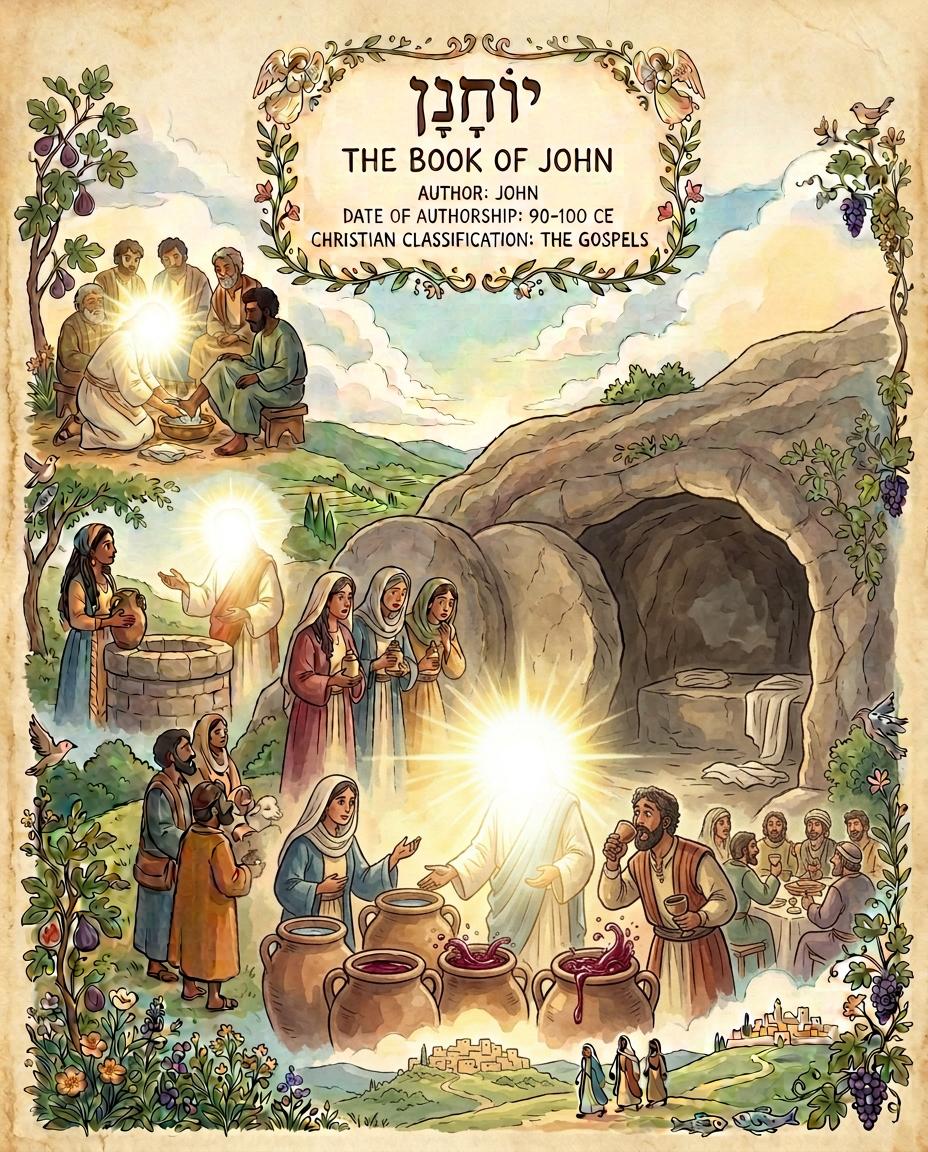
\includepdf[pages=1, fitpaper=false, width=\paperwidth, height=\paperheight, , keepaspectratio=false]{images/divider2/john2.png}
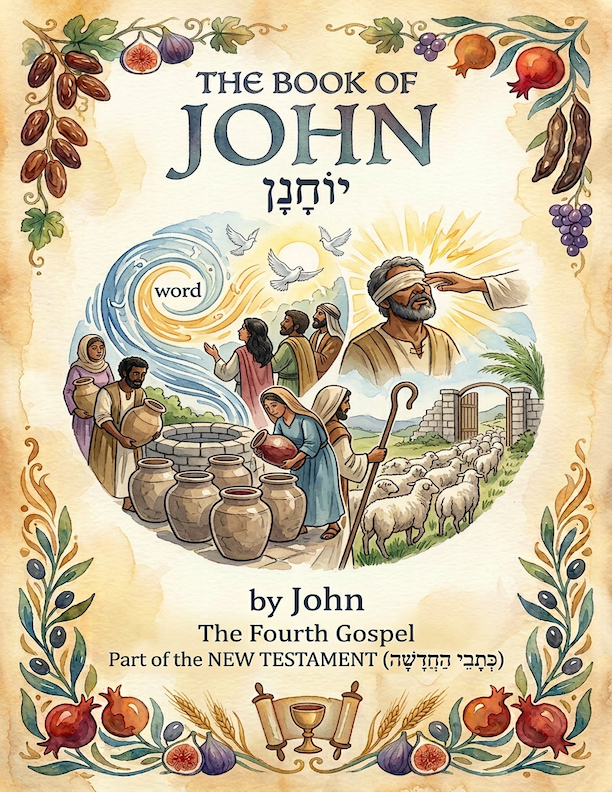
\includepdf[pages=1, fitpaper=false, width=\paperwidth, height=\paperheight, , keepaspectratio=false]{images/divider1/john.png}

\includepdf[pages=1, fitpaper=false, width=\paperwidth, height=\paperheight, , keepaspectratio=false]{images/8.5x11-Dot-Grid.png}

\includepdf[pages=1, fitpaper=false, width=\paperwidth, height=\paperheight, , keepaspectratio=false]{images/8.5x11-Dot-Grid.png}
\mybook{Yochanan}
\vspace{-1.36in}

\mychapter{} \myverse*{}In the beginning was the Word, and the Word was with God, and the
Word was God.
\myverse{}The same was in the beginning with God.
\myverse{}All things were made through him. Without him, nothing was made that has been
made.
\myverse{}In him was life, and the life was the light of men.
\myverse{}The light shines in the darkness, and the darkness hasn’t overcome\footnote{1:5 The word translated “overcome” (κατέλαβεν) can also be translated “comprehended.” It refers to
	getting a grip on an enemy to defeat him.
} it.

\myverse{}There came a man sent from God, whose name was Yochanan.
\myverse{}The same came as a witness, that he might testify about the light, that all
might believe through him.
\myverse{}He was not the light, but was sent that he might testify about the light.
\myverse{}The true light that enlightens everyone was coming into the world.

\myverse{}He was in the world, and the world was made through him, and
the world didn’t recognize him.
\myverse{}He came to his own, and those who were his own didn’t receive him.
\myverse{}But as many as received him, to them he gave the right to become God’s children,
to those who believe in his name:
\myverse{}who were born, not of blood, nor of the will of the flesh, nor of the will
of man, but of God.

\myverse{}The Word became flesh and lived among us. We saw his glory, such
glory as of the only born\footnote{1:14 The phrase “only born” is from the Greek word “μονογενους”, which is sometimes translated “only
	begotten” or “one and only”.} Son of the Father, full of grace and truth.
\myverse{}Yochanan testified about him. He cried out, saying, “This was he of whom I
said, ‘He who comes after me has surpassed me, for he was before me.’ ”
\myverse{}From his fullness we all received grace upon grace.
\myverse{}For the Torah was given through Moses. Grace and truth were realized through
Yeshua the Messiah.\footnote{1:17 “Messiah” means “Anointed One”.}
\myverse{}No one has seen God at any time. The only born\footnote{1:18 The phrase “only born” is from the Greek word “μονογενη”, which is sometimes translated “only
	begotten” or “one and only”.} Son,\footnote{1:18 NU reads “God”} who is in the bosom of the Father, has declared him.

\myverse{}This is Yochanan’s testimony, when the Judeans sent priests and
Levites from Jerusalem to ask him, “Who are you?”

\myverse{}He declared, and didn’t deny, but he declared, “I am not the
Messiah.”

\myverse{}They asked him, “What then? Are you Elijah?”

He said, “I am not.”

“Are you the prophet?”

He answered, “No.”

\myverse{}They said therefore to him, “Who are you? Give us an answer to
take back to those who sent us. What do you say about yourself?”

\myverse{}He said, “I am the voice of one crying in the wilderness, ‘Make
straight the way of the Lord,’\footnote{1:23 Isaiah 40:3} as Isaiah the prophet said.”

\myverse{}The ones who had been sent were from the Pharisees.
\myverse{}They asked him, “Why then do you immerse if you are not the Messiah, nor Elijah,
nor the prophet?”

\myverse{}Yochanan answered them, “I immerse in water, but among you stands
one whom you don’t know.
\myverse{}He is the one who comes after me, who is preferred before me, whose sandal
strap I’m not worthy to loosen.”
\myverse{}These things were done in Bethany beyond the Jordan, where Yochanan was immersing.

\myverse{}The next day, he saw Yeshua coming to him, and said, “Behold,\footnote{1:29 “Behold”, from “ἰδοὺ”, means look at, take notice, observe, see, or gaze at. It is often used
	as an interjection.} the Lamb of God, who takes away the sin of the world!
\myverse{}This is he of whom I said, ‘After me comes a man who is preferred before me,
for he was before me.’
\myverse{}I didn’t know him, but for this reason I came immersing in water, that he
would be revealed to Israel.”
\myverse{}Yochanan testified, saying, “I have seen the Spirit descending like a dove
out of heaven, and it remained on him.
\myverse{}I didn’t recognize him, but he who sent me to immerse in water said to me,
‘On whomever you will see the Spirit descending and remaining on him is he who immerses in the Holy Spirit.’
\myverse{}I have seen and have testified that this is the Son of God.”

\myverse{}Again, the next day, Yochanan was standing with two of his disciples,
\myverse{}and he looked at Yeshua as he walked, and said, “Behold, the Lamb of God!”
\myverse{}The two disciples heard him speak, and they followed Yeshua.
\myverse{}Yeshua turned and saw them following, and said to them,
\textcolor{crimson}{“What are you looking for?”}

They said to him, “Rabbi” (which is to say, being interpreted, Teacher), “where are you staying?”

\myverse{}He said to them,
\textcolor{crimson}{“Come and see.”}

They came and saw where he was staying, and they stayed with him that day. It was about the
tenth hour.\footnote{1:39 4:00 p.m.}
\myverse{}One of the two who heard Yochanan and followed him was Andrew, Simon Peter’s
brother.
\myverse{}He first found his own brother, Simon, and said to him, “We have found the
Messiah!” (which is, being interpreted, Anointed One\footnote{1:41 “Messiah” (Hebrew) and “Christ” (Greek) both mean “Anointed One”.}).
\myverse{}He brought him to Yeshua. Yeshua looked at him and said,
\textcolor{crimson}{“You are Simon the son of Jonah. You shall be called Kefa”} (which is by interpretation, Peter).\footnote{1:42 “Kefa” (Aramaic) and “Peter” (Greek) both mean “Rock”.}

\myverse{}On the next day, he was determined to go out into Galilee, and
he found Philip. Yeshua said to him,
\textcolor{crimson}{“Follow me.”}
\myverse{}Now Philip was from Bethsaida, the city of Andrew and Peter.
\myverse{}Philip found Nathanael, and said to him, “We have found him of whom Moses in the Torah
and also the prophets, wrote: Yeshua of Nazareth, the son of Joseph.”

\myverse{}Nathanael said to him, “Can any good thing come out of Nazareth?”

Philip said to him, “Come and see.”

\myverse{}Yeshua saw Nathanael coming to him, and said about him,
\textcolor{crimson}{“Behold, an Israelite indeed, in whom is no deceit!”}

\myverse{}Nathanael said to him, “How do you know me?”

Yeshua answered him,
\textcolor{crimson}{“Before Philip called you, when you were under the fig tree, I saw you.”}

\myverse{}Nathanael answered him, “Rabbi, you are the Son of God! You are
King of Israel!”

\myverse{}Yeshua answered him,
\textcolor{crimson}{“Because I told you, ‘I saw you underneath the fig tree,’ do you believe? You will see greater things
	than these!”}
\myverse{}He said to him,
\textcolor{crimson}{“Most certainly, I tell you all, hereafter you will see heaven opened, and the angels of God ascending
	and descending on the Son of Man.”}


% JOHN 2
\mychapter{} \myverse*{}The third day, there was a wedding in Cana of Galilee. Yeshua’s
mother was there.
\myverse{}Yeshua also was invited, with his disciples, to the wedding.
\myverse{}When the wine ran out, Yeshua’s mother said to him, “They have no wine.”

\myverse{}Yeshua said to her,
\textcolor{crimson}{“Woman, what does that have to do with you and me? My hour has not yet come.”}

\myverse{}His mother said to the servants, “Whatever he says to you, do it.”

\myverse{}Now there were six water pots of stone set there after the Jews’
way of purifying, containing two or three metretes\footnote{2:6 2 to 3 metretes is about 20 to 30 U. S. Gallons, or 75 to 115 liters.} apiece.
\myverse{}Yeshua said to them,
\textcolor{crimson}{“Fill the water pots with water.”} So they filled them up to the brim.
\myverse{}He said to them,
\textcolor{crimson}{“Now draw some out, and take it to the ruler of the feast.”} So they took it.
\myverse{}When the ruler of the feast tasted the water now become wine, and didn’t know
where it came from (but the servants who had drawn the water knew), the ruler of the feast called the
bridegroom
\myverse{}and said to him, “Everyone serves the good wine first, and when the guests
have drunk freely, then that which is worse. You have kept the good wine until now!”
\myverse{}This beginning of his signs Yeshua did in Cana of Galilee, and revealed his
glory; and his disciples believed in him.

\myverse{}After this, he went down to Capernaum, he, and his mother, his
brothers, and his disciples; and they stayed there a few days.

\myverse{}The Passover in Judea was at hand, and Yeshua went up to Jerusalem.
\myverse{}He found in the temple those who sold oxen, sheep, and doves, and the changers
of money sitting.
\myverse{}He made a whip of cords and drove all out of the temple, both the sheep and
the oxen; and he poured out the changers’ money and overthrew their tables.
\myverse{}To those who sold the doves, he said,
\textcolor{crimson}{“Take these things out of here! Don’t make my Father’s house a marketplace!”}
\myverse{}His disciples remembered that it was written, “Zeal for your house will eat
me up.”\footnote{2:17 Psalms 69:9}

\myverse{}The Judeans therefore answered him, “What sign do you show us,
seeing that you do these things?”

\myverse{}Yeshua answered them,
\textcolor{crimson}{“Destroy this temple, and in three days I will raise it up.”}

\myverse{}The Judeans therefore said, “It took forty-six years to build
this temple! Will you raise it up in three days?”
\myverse{}But he spoke of the temple of his body.
\myverse{}When therefore he was raised from the dead, his disciples remembered that
he said this, and they believed the Scripture and the word which Yeshua had said.

\myverse{}Now when he was in Jerusalem at the Passover, during the feast,
many believed in his name, observing his signs which he did.
\myverse{}But Yeshua didn’t entrust himself to them, because he knew everyone,
\myverse{}and because he didn’t need for anyone to testify concerning man; for he himself
knew what was in man.


% JOHN 3
\mychapter{} \myverse*{}Now there was a man of the Pharisees named Nicodemus, a ruler of the Judeans.
\myverse{}He came to Yeshua by night and said to him, “Rabbi, we know that you are a teacher
come from God, for no one can do these signs that you do, unless God is with him.”

\myverse{}Yeshua answered him,
\textcolor{crimson}{“Most certainly I tell you, unless one is born anew,
}\footnote{3:3 The word translated “anew” here and in
	Yochanan 3:7 (ἄνωθεν) also means “again” and “from above”.}
\textcolor{crimson}{he can’t see God’s Kingdom.”}

\myverse{}Nicodemus said to him, “How can a man be born when he is old? Can
he enter a second time into his mother’s womb and be born?”

\myverse{}Yeshua answered,
\textcolor{crimson}{“Most certainly I tell you, unless one is born of water and Spirit, he can’t enter into God’s Kingdom.}
\myverse{}\textcolor{crimson}{That which is born of the flesh is flesh. That which is born of the Spirit
	is spirit.
}
\myverse{}\textcolor{crimson}{Don’t marvel that I said to you, ‘You must all be born anew.’
}
\myverse{}\textcolor{crimson}{The wind}\footnote{3:8 The same Greek word (πνεῦμα) means wind, breath, and spirit.}
\textcolor{crimson}{blows where it wants to, and you hear its sound, but don’t know where it comes from and where it is
	going. So is everyone who is born of the Spirit.”}

\myverse{}Nicodemus answered him, “How can these things be?”

\myverse{}Yeshua answered him,
\textcolor{crimson}{“Are you the teacher of Israel, and don’t understand these things?
}
\myverse{}\textcolor{crimson}{Most certainly I tell you, we speak that which we know and testify of
	that which we have seen, and you don’t receive our witness.
}
\myverse{}\textcolor{crimson}{If I told you earthly things and you don’t believe, how will you believe
	if I tell you heavenly things?
}
\myverse{}\textcolor{crimson}{No one has ascended into heaven but he who descended out of heaven, the
	Son of Man, who is in heaven.
}
\myverse{}\textcolor{crimson}{As Moses lifted up the serpent in the wilderness, even so must the Son
	of Man be lifted up,
}
\myverse{}\textcolor{crimson}{that whoever believes in him should not perish, but have eternal life.
}
\myverse{}\textcolor{crimson}{For God so loved the world, that he gave his only born}\footnote{3:16 The phrase “only born” is from the Greek word “μονογενη”, which is sometimes translated “only
	begotten” or “one and only”.}
\textcolor{crimson}{Son, that whoever believes in him should not perish, but have eternal life.
}
\myverse{}\textcolor{crimson}{For God didn’t send his Son into the world to judge the world, but that
	the world should be saved through him.
}
\myverse{}\textcolor{crimson}{He who believes in him is not judged. He who doesn’t believe has been
	judged already, because he has not believed in the name of the only born Son of God.
}
\myverse{}\textcolor{crimson}{This is the judgment, that the light has come into the world, and men
	loved the darkness rather than the light, for their works were evil.
}
\myverse{}\textcolor{crimson}{For everyone who does evil hates the light and doesn’t come to the light,
	lest his works would be exposed.
}
\myverse{}\textcolor{crimson}{But he who does the truth comes to the light, that his works may be revealed,
	that they have been done in God.”}

\myverse{}After these things, Yeshua came with his disciples into the land
of Judea. He stayed there with them and immersed.
\myverse{}Yochanan also was immersing in Enon near Salim, because there was much water
there. They came and were immersed;
\myverse{}for Yochanan was not yet thrown into prison.
\myverse{}Therefore a dispute arose on the part of Yochanan’s disciples with some Judeans about purification.
\myverse{}They came to Yochanan and said to him, “Rabbi, he who was with you beyond
the Jordan, to whom you have testified, behold, he immerses, and everyone is coming to him.”

\myverse{}Yochanan answered, “A man can receive nothing unless it has been
given him from heaven.
\myverse{}You yourselves testify that I said, ‘I am not the Messiah,’ but, ‘I have been
sent before him.’
\myverse{}He who has the bride is the bridegroom; but the friend of the bridegroom,
who stands and hears him, rejoices greatly because of the bridegroom’s voice. Therefore my joy is made
full.
\myverse{}He must increase, but I must decrease.

\myverse{}“He who comes from above is above all. He who is from the earth
belongs to the earth and speaks of the earth. He who comes from heaven is above all.
\myverse{}What he has seen and heard, of that he testifies; and no one receives his
witness.
\myverse{}He who has received his witness has set his seal to this, that God is true.
\myverse{}For he whom God has sent speaks the words of God; for God gives the Spirit
without measure.
\myverse{}The Father loves the Son, and has given all things into his hand.
\myverse{}One who believes in the Son has eternal life, but one who disobeys\footnote{3:36 The same word can be translated “disobeys” or “disbelieves” in this context.} the Son
won’t see life, but the wrath of God remains on him.”


% LUKE 4
\mychapter{} \myverse*{}Therefore when the Lord knew that the Pharisees had heard that
Yeshua was making and immersing more disciples than Yochanan
\myverse{}(although Yeshua himself didn’t immerse, but his disciples),
\myverse{}he left Judea and departed into Galilee.
\myverse{}He needed to pass through Samaria.
\myverse{}So he came to a city of Samaria called Sychar, near the parcel of ground that
Jacob gave to his son Joseph.
\myverse{}Jacob’s well was there. Yeshua therefore, being tired from his journey, sat
down by the well. It was about the sixth hour.\footnote{4:6 noon}

\myverse{}A woman of Samaria came to draw water. Yeshua said to her,
\textcolor{crimson}{“Give me a drink.”}
\myverse{}For his disciples had gone away into the city to buy food.

\myverse{}The Samaritan woman therefore said to him, “How is it that you,
being a Jew, ask for a drink from me, a Samaritan woman?” (For Jews have no dealings with Samaritans.)

\myverse{}Yeshua answered her,
\textcolor{crimson}{“If you knew the gift of God, and who it is who says to you, ‘Give me a drink,’ you would have asked
	him, and he would have given you living water.”}

\myverse{}The woman said to him, “Sir, you have nothing to draw with, and
the well is deep. So where do you get that living water?
\myverse{}Are you greater than our father Jacob, who gave us the well and drank from
it himself, as did his children and his livestock?”

\myverse{}Yeshua answered her,
\textcolor{crimson}{“Everyone who drinks of this water will thirst again,
}
\myverse{}\textcolor{crimson}{but whoever drinks of the water that I will give him will never thirst
	again; but the water that I will give him will become in him a well of water springing up to eternal life.”}

\myverse{}The woman said to him, “Sir, give me this water, so that I don’t
get thirsty, neither come all the way here to draw.”

\myverse{}Yeshua said to her,
\textcolor{crimson}{“Go, call your husband, and come here.”
}

\myverse{}The woman answered, “I have no husband.”

Yeshua said to her,
\textcolor{crimson}{“You said well, ‘I have no husband,’
}
\myverse{}\textcolor{crimson}{for you have had five husbands; and he whom you now have is not your husband.
	This you have said truly.”}

\myverse{}The woman said to him, “Sir, I perceive that you are a prophet.
\myverse{}Our fathers worshiped in this mountain, and you Jews say that in Jerusalem
is the place where people ought to worship.”

\myverse{}Yeshua said to her,
\textcolor{crimson}{“Woman, believe me, the hour is coming when neither in this mountain nor in Jerusalem will you worship
	the Father.
}
\myverse{}\textcolor{crimson}{You worship that which you don’t know. We worship that which we know;
	for salvation is from the Jews.
}
\myverse{}\textcolor{crimson}{But the hour comes, and now is, when the true worshipers will worship
	the Father in spirit and truth, for the Father seeks such to be his worshipers.
}
\myverse{}\textcolor{crimson}{God is spirit, and those who worship him must worship in spirit and truth.”}

\myverse{}The woman said to him, “I know that Messiah is coming, he who
is called Messiah.\footnote{4:25 “Messiah” (Hebrew) and “Christ” (Greek) both mean “Anointed One”.} When he has come,
he will declare to us all things.”

\myverse{}Yeshua said to her,
\textcolor{crimson}{“I am he, the one who speaks to you.”}

\myverse{}Just then, his disciples came. They marveled that he was speaking
with a woman; yet no one said, “What are you looking for?” or, “Why do you speak with her?”
\myverse{}So the woman left her water pot, went away into the city, and said to the
people,
\myverse{}“Come, see a man who told me everything that I have done. Can this be the
Messiah?”
\myverse{}They went out of the city, and were coming to him.

\myverse{}In the meanwhile, the disciples urged him, saying, “Rabbi, eat.”

\myverse{}But he said to them,
\textcolor{crimson}{“I have food to eat that you don’t know about.”}

\myverse{}The disciples therefore said to one another, “Has anyone brought
him something to eat?”

\myverse{}Yeshua said to them,
\textcolor{crimson}{“My food is to do the will of him who sent me and to accomplish his work.
}
\myverse{}\textcolor{crimson}{Don’t you say, ‘There are yet four months until the harvest’? Behold,
	I tell you, lift up your eyes and look at the fields, that they are white for harvest already.
}
\myverse{}\textcolor{crimson}{He who reaps receives wages and gathers fruit to eternal life, that both
	he who sows and he who reaps may rejoice together.
}
\myverse{}\textcolor{crimson}{For in this the saying is true, ‘One sows, and another reaps.’
}
\myverse{}\textcolor{crimson}{I sent you to reap that for which you haven’t labored. Others have labored,
	and you have entered into their labor.”}

\myverse{}From that city many of the Samaritans believed in him because
of the word of the woman, who testified, “He told me everything that I have done.”
\myverse{}So when the Samaritans came to him, they begged him to stay with them. He
stayed there two days.
\myverse{}Many more believed because of his word.
\myverse{}They said to the woman, “Now we believe, not because of your speaking; for
we have heard for ourselves, and know that this is indeed the Messiah, the Savior of the world.”

\myverse{}After the two days he went out from there and went into Galilee.
\myverse{}For Yeshua himself testified that a prophet has no honor in his own country.
\myverse{}So when he came into Galilee, the Galileans received him, having seen all
the things that he did in Jerusalem at the feast, for they also went to the feast.
\myverse{}Yeshua came therefore again to Cana of Galilee, where he made the water into
wine. There was a certain nobleman whose son was sick at Capernaum.
\myverse{}When he heard that Yeshua had come out of Judea into Galilee, he went to him
and begged him that he would come down and heal his son, for he was at the point of death.
\myverse{}Yeshua therefore said to him,
\textcolor{crimson}{“Unless you people see signs and wonders, you will in no way believe.”}

\myverse{}The nobleman said to him, “Sir, come down before my child dies.”

\myverse{}Yeshua said to him,
\textcolor{crimson}{“Go your way. Your son lives.”} The man believed the word that Yeshua spoke to him, and he went
his way.
\myverse{}As he was going down, his servants met him and reported, saying “Your child
lives!”
\myverse{}So he inquired of them the hour when he began to get better. They said therefore
to him, “Yesterday at the seventh hour,\footnote{4:52 1:00 p.m.} the fever left him.”
\myverse{}So the father knew that it was at that hour in which Yeshua said to him,
\textcolor{crimson}{“Your son lives.”} He believed, as did his whole house.
\myverse{}This is again the second sign that Yeshua did, having come out of Judea into
Galilee.


% JOHN 5
\mychapter{} \myverse*{}After these things, there was a Jewish festival, and Yeshua went
up to Jerusalem.
\myverse{}Now in Jerusalem by the sheep gate, there is a pool, which is called in Hebrew,
“Bethesda”, having five porches.
\myverse{}In these lay a great multitude of those who were sick, blind, lame, or paralyzed,
waiting for the moving of the water;
\myverse{}for an angel went down at certain times into the pool and stirred up the water.
Whoever stepped in first after the stirring of the water was healed of whatever disease he had.\footnote{5:4 NU omits from “waiting” in verse 3 to the end of verse 4.}
\myverse{}A certain man was there who had been sick for thirty-eight years.
\myverse{}When Yeshua saw him lying there, and knew that he had been sick for a long time,
he asked him,
\textcolor{crimson}{“Do you want to be made well?”}

\myverse{}The sick man answered him, “Sir, I have no one to put me into the
pool when the water is stirred up, but while I’m coming, another steps down before me.”

\myverse{}Yeshua said to him,
\textcolor{crimson}{“Arise, take up your mat, and walk.”}

\myverse{}Immediately, the man was made well, and took up his mat and walked.

Now that day was a Sabbath.
\myverse{}So the Judeans said to him who was cured, “It is the Sabbath. It is not lawful
for you to carry the mat.”

\myverse{}He answered them, “He who made me well said to me,
\textcolor{crimson}{‘Take up your mat and walk.’} ”

\myverse{}Then they asked him, “Who is the man who said to you,
\textcolor{crimson}{‘Take up your mat and walk’}?”

\myverse{}But he who was healed didn’t know who it was, for Yeshua had
withdrawn, a crowd being in the place.

\myverse{}Afterward Yeshua found him in the temple and said to him,
\textcolor{crimson}{“Behold, you are made well. Sin no more, so that nothing worse happens to you.”
}

\myverse{}The man went away, and told the Judeans that it was Yeshua who
had made him well.
\myverse{}For this cause the Judeans persecuted Yeshua and sought to kill him, because
he did these things on the Sabbath.
\myverse{}But Yeshua answered them,
\textcolor{crimson}{“My Father is still working, so I am working, too.”}

\myverse{}For this cause therefore the Judeans sought all the more to kill
him, because he not only broke the Sabbath, but also called God his own Father, making himself equal with
God.
\myverse{}Yeshua therefore answered them,
\textcolor{crimson}{“Most certainly, I tell you, the Son can do nothing of himself, but what he sees the Father doing.
	For whatever things he does, these the Son also does likewise.
}
\myverse{}\textcolor{crimson}{For the Father has affection for the Son, and shows him all things that
	he himself does. He will show him greater works than these, that you may marvel.
}
\myverse{}\textcolor{crimson}{For as the Father raises the dead and gives them life, even so the Son
	also gives life to whom he desires.
}
\myverse{}\textcolor{crimson}{For the Father judges no one, but he has given all judgment to the Son,
}
\myverse{}\textcolor{crimson}{that all may honor the Son, even as they honor the Father. He who doesn’t
	honor the Son doesn’t honor the Father who sent him.}

\myverse{}\textcolor{crimson}{“Most certainly I tell you, he who hears my word and believes
	him who sent me has eternal life, and doesn’t come into judgment, but has passed out of death into life.
}
\myverse{}\textcolor{crimson}{Most certainly I tell you, the hour comes, and now is, when the dead will
	hear the Son of God’s voice; and those who hear will live.
}
\myverse{}\textcolor{crimson}{For as the Father has life in himself, even so he gave to the Son also
	to have life in himself.
}
\myverse{}\textcolor{crimson}{He also gave him authority to execute judgment, because he is a son of
	man.
}
\myverse{}\textcolor{crimson}{Don’t marvel at this, for the hour comes in which all who are in the tombs
	will hear his voice
}
\myverse{}\textcolor{crimson}{and will come out; those who have done good, to the resurrection of life;
	and those who have done evil, to the resurrection of judgment.
}
\myverse{}\textcolor{crimson}{I can of myself do nothing. As I hear, I judge; and my judgment is righteous,
	because I don’t seek my own will, but the will of my Father who sent me.}

\myverse{}\textcolor{crimson}{“If I testify about myself, my witness is not valid.} \myverse{}\textcolor{crimson}{It is another who testifies about me. I know that the testimony which he testifies about me is true.} \myverse{}\textcolor{crimson}{You have sent to Yochanan, and he has testified to the truth.} \myverse{}\textcolor{crimson}{But the testimony which I receive is not from man. However, I say these things that you may be saved.} \myverse{}\textcolor{crimson}{He was the burning and shining lamp, and you were willing to rejoice for a while in his light.}
\myverse{}\textcolor{crimson}{But the testimony which I have is greater than that of Yochanan; for the
	works which the Father gave me to accomplish, the very works that I do, testify about me, that the Father
	has sent me.
}
\myverse{}\textcolor{crimson}{The Father himself, who sent me, has testified about me. You have neither
	heard his voice at any time, nor seen his form.
}
\myverse{}\textcolor{crimson}{You don’t have his word living in you, because you don’t believe him whom
	he sent.}

\myverse{}\textcolor{crimson}{“You search the Scriptures, because you think that in them
	you have eternal life; and these are they which testify about me.
}
\myverse{}\textcolor{crimson}{Yet you will not come to me, that you may have life.
}
\myverse{}\textcolor{crimson}{I don’t receive glory from men.
}
\myverse{}\textcolor{crimson}{But I know you, that you don’t have God’s love in yourselves.
}
\myverse{}\textcolor{crimson}{I have come in my Father’s name, and you don’t receive me. If another
	comes in his own name, you will receive him.
}
\myverse{}\textcolor{crimson}{How can you believe, who receive glory from one another, and you don’t
	seek the glory that comes from the only God?}

\myverse{}\textcolor{crimson}{“Don’t think that I will accuse you to the Father. There
	is one who accuses you, even Moses, on whom you have set your hope.
}
\myverse{}\textcolor{crimson}{For if you believed Moses, you would believe me; for he wrote about me.
}
\myverse{}\textcolor{crimson}{But if you don’t believe his writings, how will you believe my words?”}


% JOHN 6
\mychapter{} \myverse*{}After these things, Yeshua went away to the other side of the sea
of Galilee, which is also called the Sea of Tiberias.
\myverse{}A great multitude followed him, because they saw his signs which he did on those
who were sick.
\myverse{}Yeshua went up into the mountain, and he sat there with his disciples.
\myverse{}Now the Passover, the Jewish festival, was at hand.
\myverse{}Yeshua therefore, lifting up his eyes and seeing that a great multitude was
coming to him, said to Philip,
\textcolor{crimson}{“Where are we to buy bread, that these may eat?”}
\myverse{}He said this to test him, for he himself knew what he would do.

\myverse{}Philip answered him, “Two hundred denarii\footnote{6:7 A denarius was a silver coin worth about a day’s wages for an agricultural laborer, so 200 denarii
	would be between 6 and 7 month’s pay.} worth of bread is not sufficient for them, that every one
of them may receive a little.”

\myverse{}One of his disciples, Andrew, Simon Peter’s brother, said to him,
\myverse{}“There is a boy here who has five barley loaves and two fish, but what are these
among so many?”

\myverse{}Yeshua said,
\textcolor{crimson}{“Have the people sit down.”} Now there was much grass in that place. So the men sat down, in number
about five thousand.
\myverse{}Yeshua took the loaves, and having given thanks, he distributed to the disciples,
and the disciples to those who were sitting down, likewise also of the fish as much as they desired.
\myverse{}When they were filled, he said to his disciples,
\textcolor{crimson}{“Gather up the broken pieces which are left over, that nothing be lost.”}
\myverse{}So they gathered them up, and filled twelve baskets with broken pieces from
the five barley loaves, which were left over by those who had eaten.
\myverse{}When therefore the people saw the sign which Yeshua did, they said, “This
is truly the Prophet who comes into the world.”
\myverse{}Yeshua therefore, perceiving that they were about to come and take him by
force to make him king, withdrew again to the mountain by himself.

\myverse{}When evening came, his disciples went down to the sea.
\myverse{}They entered into the boat, and were going over the sea to Capernaum. It was
now dark, and Yeshua had not come to them.
\myverse{}The sea was tossed by a great wind blowing.
\myverse{}When therefore they had rowed about twenty-five or thirty stadia,\footnote{6:19 25 to 30 stadia is about 5 to 6 kilometers or about 3 to 4 miles} they saw Yeshua walking
on the sea\footnote{6:19 See
	Job 9:8} and drawing near to the boat; and they were afraid.
\myverse{}But he said to them,
\textcolor{crimson}{“It is I.}\footnote{6:20 or, I AM}
\textcolor{crimson}{Don’t be afraid.”}
\myverse{}They were willing therefore to receive him into the boat. Immediately the
boat was at the land where they were going.

\myverse{}On the next day, the multitude that stood on the other side of
the sea saw that there was no other boat there, except the one in which his disciples had embarked, and
that Yeshua hadn’t entered with his disciples into the boat, but his disciples had gone away alone.
\myverse{}However, boats from Tiberias came near to the place where they ate the bread
after the Lord had given thanks.
\myverse{}When the multitude therefore saw that Yeshua wasn’t there, nor his disciples,
they themselves got into the boats and came to Capernaum, seeking Yeshua.
\myverse{}When they found him on the other side of the sea, they asked him, “Rabbi,
when did you come here?”

\myverse{}Yeshua answered them,
\textcolor{crimson}{“Most certainly I tell you, you seek me, not because you saw signs, but because you ate of the loaves
	and were filled.
}
\myverse{}\textcolor{crimson}{Don’t work for the food which perishes, but for the food which remains
	to eternal life, which the Son of Man will give to you. For God the Father has sealed him.”}

\myverse{}They said therefore to him, “What must we do, that we may work
the works of God?”

\myverse{}Yeshua answered them,
\textcolor{crimson}{“This is the work of God, that you believe in him whom he has sent.”}

\myverse{}They said therefore to him, “What then do you do for a sign,
that we may see and believe you? What work do you do?
\myverse{}Our fathers ate the manna in the wilderness. As it is written, ‘He gave them
bread out of heaven\footnote{6:31 Greek and Hebrew use the same word for “heaven”, “the heavens”, “the sky”, and “the air”.}
to eat.’ ”\footnote{6:31 Exodus 16:4;
	Nehemiah 9:15;
	Psalms 78:24-25}

\myverse{}Yeshua therefore said to them,
\textcolor{crimson}{“Most certainly, I tell you, it wasn’t Moses who gave you the bread out of heaven, but my Father gives
	you the true bread out of heaven.
}
\myverse{}\textcolor{crimson}{For the bread of God is that which comes down out of heaven and gives
	life to the world.”}

\myverse{}They said therefore to him, “Lord, always give us this bread.”

\myverse{}Yeshua said to them,
\textcolor{crimson}{“I am the bread of life. Whoever comes to me will not be hungry, and whoever believes in me will never
	be thirsty.
}
\myverse{}\textcolor{crimson}{But I told you that you have seen me, and yet you don’t believe.
}
\myverse{}\textcolor{crimson}{All those whom the Father gives me will come to me. He who comes to me
	I will in no way throw out.
}
\myverse{}\textcolor{crimson}{For I have come down from heaven, not to do my own will, but the will
	of him who sent me.
}
\myverse{}\textcolor{crimson}{This is the will of my Father who sent me, that of all he has given to
	me I should lose nothing, but should raise him up at the last day.
}
\myverse{}\textcolor{crimson}{This is the will of the one who sent me, that everyone who sees the Son
	and believes in him should have eternal life; and I will raise him up at the last day.”}

\myverse{}The Judeans therefore murmured concerning him, because he said,
\textcolor{crimson}{“I am the bread which came down out of heaven.”}
\myverse{}They said, “Isn’t this Yeshua, the son of Joseph, whose father and mother
we know? How then does he say,
\textcolor{crimson}{‘I have come down out of heaven’?”
}

\myverse{}Therefore Yeshua answered them,
\textcolor{crimson}{“Don’t murmur among yourselves.
}
\myverse{}\textcolor{crimson}{No one can come to me unless the Father who sent me draws him; and I will
	raise him up in the last day.
}
\myverse{}\textcolor{crimson}{It is written in the Prophets, ‘They will all be taught by God.’
}\footnote{6:45 Isaiah 54:13}
\textcolor{crimson}{Therefore everyone who hears from the Father and has learned, comes to me.
}
\myverse{}\textcolor{crimson}{Not that anyone has seen the Father, except he who is from God. He has
	seen the Father.
}
\myverse{}\textcolor{crimson}{Most certainly, I tell you, he who believes in me has eternal life.
}
\myverse{}\textcolor{crimson}{I am the bread of life.
}
\myverse{}\textcolor{crimson}{Your fathers ate the manna in the wilderness and they died.
}
\myverse{}\textcolor{crimson}{This is the bread which comes down out of heaven, that anyone may eat
	of it and not die.
}
\myverse{}\textcolor{crimson}{I am the living bread which came down out of heaven. If anyone eats of
	this bread, he will live forever. Yes, the bread which I will give for the life of the world is my flesh.”}

\myverse{}The Judeans therefore contended with one another, saying, “How
can this man give us his flesh to eat?”

\myverse{}Yeshua therefore said to them,
\textcolor{crimson}{“Most certainly I tell you, unless you eat the flesh of the Son of Man and drink his blood, you don’t
	have life in yourselves.
}
\myverse{}\textcolor{crimson}{He who eats my flesh and drinks my blood has eternal life, and I will
	raise him up at the last day.
}
\myverse{}\textcolor{crimson}{For my flesh is food indeed, and my blood is drink indeed.
}
\myverse{}\textcolor{crimson}{He who eats my flesh and drinks my blood lives in me, and I in him.
}
\myverse{}\textcolor{crimson}{As the living Father sent me, and I live because of the Father, so he
	who feeds on me will also live because of me.
}
\myverse{}\textcolor{crimson}{This is the bread which came down out of heaven—not as our fathers ate
	the manna and died. He who eats this bread will live forever.”}
\myverse{}He said these things in the synagogue, as he taught in Capernaum.

\myverse{}Therefore many of his disciples, when they heard this, said,
“This is a hard saying! Who can listen to it?”

\myverse{}But Yeshua knowing in himself that his disciples murmured at
this, said to them,
\textcolor{crimson}{“Does this cause you to stumble?
}
\myverse{}\textcolor{crimson}{Then what if you would see the Son of Man ascending to where he was before?
}
\myverse{}\textcolor{crimson}{It is the spirit who gives life. The flesh profits nothing. The words
	that I speak to you are spirit, and are life.
}
\myverse{}\textcolor{crimson}{But there are some of you who don’t believe.”} For Yeshua knew from
the beginning who they were who didn’t believe, and who it was who would betray him.
\myverse{}He said,
\textcolor{crimson}{“For this cause I have said to you that no one can come to me, unless it is given to him by my Father.”}

\myverse{}At this, many of his disciples went back and walked no more with
him.
\myverse{}Yeshua said therefore to the twelve,
\textcolor{crimson}{“You don’t also want to go away, do you?”}

\myverse{}Simon Peter answered him, “Lord, to whom would we go? You have
the words of eternal life.
\myverse{}We have come to believe and know that you are the Messiah, the Son of the
living God.”

\myverse{}Yeshua answered them,
\textcolor{crimson}{“Didn’t I choose you, the twelve, and one of you is a devil?”}
\myverse{}Now he spoke of Judah, the son of Simon Iscariot, for it was he who would
betray him, being one of the twelve.


% JOHN 7
\mychapter{} \myverse*{}After these things, Yeshua was walking in Galilee, for he wouldn’t
walk in Judea, because the Judeans sought to kill him.
\myverse{}Now the Jewish festival, the Feast of Sukkot, was at hand.
\myverse{}His brothers therefore said to him, “Depart from here and go into Judea, that
your disciples also may see your works which you do.
\myverse{}For no one does anything in secret while he seeks to be known openly. If you
do these things, reveal yourself to the world.”
\myverse{}For even his brothers didn’t believe in him.

\myverse{}Yeshua therefore said to them,
\textcolor{crimson}{“My time has not yet come, but your time is always ready.
}
\myverse{}\textcolor{crimson}{The world can’t hate you, but it hates me, because I testify about it, that
	its works are evil.
}
\myverse{}\textcolor{crimson}{You go up to the feast. I am not yet going up to this feast, because my
	time is not yet fulfilled.”}

\myverse{}Having said these things to them, he stayed in Galilee.
\myverse{}But when his brothers had gone up to the feast, then he also went up, not
publicly, but as it were in secret.
\myverse{}The Judeans therefore sought him at the feast, and said, “Where is he?”
\myverse{}There was much murmuring among the multitudes concerning him. Some said, “He
is a good man.” Others said, “Not so, but he leads the multitude astray.”
\myverse{}Yet no one spoke openly of him for fear of the Judeans.
\myverse{}But when it was now the middle of the feast, Yeshua went up into the temple
and taught.
\myverse{}The Judeans therefore marveled, saying, “How does this man know letters, having
never been educated?”

\myverse{}Yeshua therefore answered them,
\textcolor{crimson}{“My teaching is not mine, but his who sent me.
}
\myverse{}\textcolor{crimson}{If anyone desires to do his will, he will know about the teaching, whether
	it is from God or if I am speaking from myself.
}
\myverse{}\textcolor{crimson}{He who speaks from himself seeks his own glory, but he who seeks the glory
	of him who sent him is true, and no unrighteousness is in him.
}
\myverse{}\textcolor{crimson}{Didn’t Moses give you the Torah, and yet none of you keeps the Torah?
	Why do you seek to kill me?”}

\myverse{}The multitude answered, “You have a demon! Who seeks to kill
you?”

\myverse{}Yeshua answered them,
\textcolor{crimson}{“I did one work and you all marvel because of it.
}
\myverse{}\textcolor{crimson}{Moses has given you circumcision (not that it is of Moses, but of the
	fathers), and on the Sabbath you circumcise a boy.
}
\myverse{}\textcolor{crimson}{If a boy receives circumcision on the Sabbath, that the Torah of Moses
	may not be broken, are you angry with me because I made a man completely healthy on the Sabbath?
}
\myverse{}\textcolor{crimson}{Don’t judge according to appearance, but judge righteous judgment.”
}

\myverse{}Therefore some of them of Jerusalem said, “Isn’t this he whom
they seek to kill?
\myverse{}Behold, he speaks openly, and they say nothing to him. Can it be that the
rulers indeed know that this is truly the Messiah?
\myverse{}However, we know where this man comes from, but when the Messiah comes, no
one will know where he comes from.”

\myverse{}Yeshua therefore cried out in the temple, teaching and saying,
\textcolor{crimson}{“You both know me, and know where I am from. I have not come of myself, but he who sent me is true,
	whom you don’t know.
}
\myverse{}\textcolor{crimson}{I know him, because I am from him, and he sent me.”}

\myverse{}They sought therefore to take him; but no one laid a hand on
him, because his hour had not yet come.
\myverse{}But of the multitude, many believed in him. They said, “When the Messiah comes,
he won’t do more signs than those which this man has done, will he?”
\myverse{}The Pharisees heard the multitude murmuring these things concerning him, and
the chief priests and the Pharisees sent officers to arrest him.

\myverse{}Then Yeshua said,
\textcolor{crimson}{“I will be with you a little while longer, then I go to him who sent me.
}
\myverse{}\textcolor{crimson}{You will seek me and won’t find me. You can’t come where I am.”}

\myverse{}The Judeans therefore said among themselves, “Where will this
man go that we won’t find him? Will he go to the Diaspora among the Greeks and teach the Greeks?
\myverse{}What is this word that he said,
\textcolor{crimson}{‘You will seek me, and won’t find me;’} and
\textcolor{crimson}{‘Where I am, you can’t come’}?”

\myverse{}Now on the last and greatest day of the feast\footnote{7:37 Known today as Hoshana Rabbah.},
Yeshua stood and cried out,
\textcolor{crimson}{“If anyone is thirsty, let him come to me and drink!
}
\myverse{}\textcolor{crimson}{He who believes in me, as the Scripture has said, from within him will
	flow rivers of living water.”}
\myverse{}But he said this about the Spirit, which those believing in him were to receive.
For the Holy Spirit was not yet given, because Yeshua wasn’t yet glorified.

\myverse{}Many of the multitude therefore, when they heard these words,
said, “This is truly the Prophet.”
\myverse{}Others said, “This is the Messiah.” But some said, “What, does the Messiah
come out of Galilee?
\myverse{}Hasn’t the Scripture said that the Messiah comes of the offspring\footnote{7:42 or, seed} of David,\footnote{7:42 2 Samuel 7:12} and from Bethlehem,\footnote{7:42 Micah 5:2} the village where David was?”
\myverse{}So a division arose in the multitude because of him.
\myverse{}Some of them would have arrested him, but no one laid hands on him.
\myverse{}The officers therefore came to the chief priests and Pharisees; and they said
to them, “Why didn’t you bring him?”

\myverse{}The officers answered, “No man ever spoke like this man!”

\myverse{}The Pharisees therefore answered them, “You aren’t also led astray,
are you?
\myverse{}Have any of the rulers or any of the Pharisees believed in him?
\myverse{}But this multitude that doesn’t know the Torah is cursed.”

\myverse{}Nicodemus (he who came to him by night, being one of them) said
to them,
\myverse{}“Does our Torah judge a man unless it first hears from him personally and
knows what he does?”

\myverse{}They answered him, “Are you also from Galilee? Search and see
that no prophet has arisen out of Galilee.”\footnote{7:52 See
	Isaiah 9:1;
	Matthew 4:13-16}

\myverse{}Everyone went to his own house,

%JOHN 8
\mychapter{}\myverse*{}but Yeshua went to the Mount of Olives.

\myverse{}Now very early in the morning, he came again into the temple, and
all the people came to him. He sat down and taught them.
\myverse{}The scribes and the Pharisees brought a woman taken in adultery. Having set
her in the middle,
\myverse{}they told him, “Rabbi, we found this woman in adultery, in the very act.
\myverse{}Now in our Torah, Moses commanded us to stone such women.\footnote{8:5 Leviticus 20:10;
	Deuteronomy 22:22} What then do you say about her?”
\myverse{}They said this testing him, that they might have something to accuse him of.

But Yeshua stooped down and wrote on the ground with his finger.
\myverse{}But when they continued asking him, he looked up and said to them,
\textcolor{crimson}{“He who is without sin among you, let him throw the first stone at her.”
}
\myverse{}Again he stooped down and wrote on the ground with his finger.

\myverse{}They, when they heard it, being convicted by their conscience,
went out one by one, beginning from the oldest, even to the last. Yeshua was left alone with the woman
where she was, in the middle.
\myverse{}Yeshua, standing up, saw her and said,
\textcolor{crimson}{“Woman, where are your accusers? Did no one condemn you?”}

\myverse{}She said, “No one, Lord.”

Yeshua said,
\textcolor{crimson}{“Neither do I condemn you. Go your way. From now on, sin no more.”}\footnote{8:11 NU includes
	Yochanan 7:53–Yochanan 8:11, but puts brackets around
	it to indicate that the textual critics had less confidence that this was original.}

\myverse{}Again, therefore, Yeshua spoke to them, saying,
\textcolor{crimson}{“I am the light of the world.}\footnote{8:12 Isaiah 60:1}
\textcolor{crimson}{He who follows me will not walk in the darkness, but will have the light of life.”}

\myverse{}The Pharisees therefore said to him, “You testify about yourself.
Your testimony is not valid.”

\myverse{}Yeshua answered them,
\textcolor{crimson}{“Even if I testify about myself, my testimony is true, for I know where I came from, and where I am
	going; but you don’t know where I came from, or where I am going.
}
\myverse{}\textcolor{crimson}{You judge according to the flesh. I judge no one.
}
\myverse{}\textcolor{crimson}{Even if I do judge, my judgment is true, for I am not alone, but I am
	with the Father who sent me.
}
\myverse{}\textcolor{crimson}{It’s also written in your Torah that the testimony of two people is valid.}\footnote{8:17 Deuteronomy 17:6;
	19:15}
\myverse{}\textcolor{crimson}{I am one who testifies about myself, and the Father who sent me testifies
	about me.”}

\myverse{}They said therefore to him, “Where is your Father?”

Yeshua answered,
\textcolor{crimson}{“You know neither me nor my Father. If you knew me, you would know my Father also.”}
\myverse{}Yeshua spoke these words in the treasury, as he taught in the temple. Yet
no one arrested him, because his hour had not yet come.
\myverse{}Yeshua said therefore again to them,
\textcolor{crimson}{“I am going away, and you will seek me, and you will die in your sins. Where I go, you can’t come.”
}

\myverse{}The Judeans therefore said, “Will he kill himself, because he
says,
\textcolor{crimson}{‘Where I am going, you can’t come’}?”

\myverse{}He said to them,
\textcolor{crimson}{“You are from beneath. I am from above. You are of this world. I am not of this world.
}
\myverse{}\textcolor{crimson}{I said therefore to you that you will die in your sins; for unless you
	believe that I am}\footnote{8:24 or, I AM}
\textcolor{crimson}{he, you will die in your sins.”
}

\myverse{}They said therefore to him, “Who are you?”

Yeshua said to them,
\textcolor{crimson}{“Just what I have been saying to you from the beginning.
}
\myverse{}\textcolor{crimson}{I have many things to speak and to judge concerning you. However, he who
	sent me is true; and the things which I heard from him, these I say to the world.”}

\myverse{}They didn’t understand that he spoke to them about the Father.
\myverse{}Yeshua therefore said to them,
\textcolor{crimson}{“When you have lifted up the Son of Man, then you will know that I am he, and I do nothing of myself,
	but as my Father taught me, I say these things.
}
\myverse{}\textcolor{crimson}{He who sent me is with me. The Father hasn’t left me alone, for I always
	do the things that are pleasing to him.”}

\myverse{}As he spoke these things, many believed in him.
\myverse{}Yeshua therefore said to those Judeans who had believed him,
\textcolor{crimson}{“If you remain in my word, then you are truly my disciples.
}
\myverse{}\textcolor{crimson}{You will know the truth, and the truth will make you free.”
}\footnote{8:32 Psalms 119:45}

\myverse{}They answered him, “We are Abraham’s offspring, and have never
been in bondage to anyone. How do you say,
\textcolor{crimson}{‘You will be made free’}?”

\myverse{}Yeshua answered them,
\textcolor{crimson}{“Most certainly I tell you, everyone who commits sin is the bondservant of sin.
}
\myverse{}\textcolor{crimson}{A bondservant doesn’t live in the house forever. A son remains forever.
}
\myverse{}\textcolor{crimson}{If therefore the Son makes you free, you will be free indeed.
}
\myverse{}\textcolor{crimson}{I know that you are Abraham’s offspring, yet you seek to kill me, because
	my word finds no place in you.
}
\myverse{}\textcolor{crimson}{I say the things which I have seen with my Father; and you also do the
	things which you have seen with your father.”}

\myverse{}They answered him, “Our father is Abraham.”

Yeshua said to them,
\textcolor{crimson}{“If you were Abraham’s children, you would do the works of Abraham.
}
\myverse{}\textcolor{crimson}{But now you seek to kill me, a man who has told you the truth which I
	heard from God. Abraham didn’t do this.
}
\myverse{}\textcolor{crimson}{You do the works of your father.”}

They said to him, “We were not born of sexual immorality. We have one Father, God.”

\myverse{}Therefore Yeshua said to them,
\textcolor{crimson}{“If God were your father, you would love me, for I came out and have come from God. For I haven’t
	come of myself, but he sent me.
}
\myverse{}\textcolor{crimson}{Why don’t you understand my speech? Because you can’t hear my word.
}
\myverse{}\textcolor{crimson}{You are of your father the devil, and you want to do the desires of your
	father. He was a murderer from the beginning, and doesn’t stand in the truth, because there is no truth
	in him. When he speaks a lie, he speaks on his own; for he is a liar, and the father of lies.
}
\myverse{}\textcolor{crimson}{But because I tell the truth, you don’t believe me.
}
\myverse{}\textcolor{crimson}{Which of you convicts me of sin? If I tell the truth, why do you not believe
	me?
}
\myverse{}\textcolor{crimson}{He who is of God hears the words of God. For this cause you don’t hear,
	because you are not of God.”}

\myverse{}Then the Judeans answered him, “Don’t we say well that you are
a Samaritan, and have a demon?”

\myverse{}Yeshua answered,
\textcolor{crimson}{“I don’t have a demon, but I honor my Father and you dishonor me.
}
\myverse{}\textcolor{crimson}{But I don’t seek my own glory. There is one who seeks and judges.
}
\myverse{}\textcolor{crimson}{Most certainly, I tell you, if a person keeps my word, he will never see
	death.”}

\myverse{}Then the Judeans said to him, “Now we know that you have a demon.
Abraham died, as did the prophets; and you say,
\textcolor{crimson}{‘If a man keeps my word, he will never taste of death.’}
\myverse{}Are you greater than our father Abraham, who died? The prophets died. Who
do you make yourself out to be?”

\myverse{}Yeshua answered,
\textcolor{crimson}{“If I glorify myself, my glory is nothing. It is my Father who glorifies me, of whom you say that
	he is our God.
}
\myverse{}\textcolor{crimson}{You have not known him, but I know him. If I said, ‘I don’t know him,’
	I would be like you, a liar. But I know him and keep his word.
}
\myverse{}\textcolor{crimson}{Your father Abraham rejoiced to see my day. He saw it and was glad.”}

\myverse{}The Judeans therefore said to him, “You are not yet fifty years
old! Have you seen Abraham?”

\myverse{}Yeshua said to them,
\textcolor{crimson}{“Most certainly, I tell you, before Abraham came into existence, I AM.}\footnote{8:58 Exodus 3:14}\textcolor{crimson}{”}

\myverse{}Therefore they took up stones to throw at him, but Yeshua hid
himself and went out of the temple, having gone through the middle of them, and so passed by.


% JOHN 9
\mychapter{} \myverse*{}As he passed by, he saw a man blind from birth.
\myverse{}His disciples asked him, “Rabbi, who sinned, this man or his parents, that he
was born blind?”

\myverse{}Yeshua answered,
\textcolor{crimson}{“This man didn’t sin, nor did his parents, but that the works of God might be revealed in him.
}
\myverse{}\textcolor{crimson}{I must work the works of him who sent me while it is day. The night is coming,
	when no one can work.
}
\myverse{}\textcolor{crimson}{While I am in the world, I am the light of the world.”}
\myverse{}When he had said this, he spat on the ground, made mud with the saliva, anointed
the blind man’s eyes with the mud,
\myverse{}and said to him,
\textcolor{crimson}{“Go, wash in the pool of Siloam”} (which means “Sent”). So he went away, washed, and came back
seeing.

\myverse{}Therefore the neighbors and those who saw that he was blind before
said, “Isn’t this he who sat and begged?”
\myverse{}Others were saying, “It is he.” Still others were saying, “He looks like him.”

He said, “I am he.”

\myverse{}They therefore were asking him, “How were your eyes opened?”

\myverse{}He answered, “A man called Yeshua made mud, anointed my eyes,
and said to me,
\textcolor{crimson}{‘Go to the pool of Siloam and wash.’} So I went away and washed, and I received sight.”

\myverse{}Then they asked him, “Where is he?”

He said, “I don’t know.”

\myverse{}They brought him who had been blind to the Pharisees.
\myverse{}It was a Sabbath when Yeshua made the mud and opened his eyes.
\myverse{}Again therefore the Pharisees also asked him how he received his sight. He
said to them, “He put mud on my eyes, I washed, and I see.”

\myverse{}Some therefore of the Pharisees said, “This man is not from God,
because he doesn’t keep the Sabbath.”

Others said, “How can a man who is a sinner do such signs?” So there was division among them.

\myverse{}Therefore they asked the blind man again, “What do you say about
him, because he opened your eyes?”

He said, “He is a prophet.”

\myverse{}The Judeans therefore didn’t believe concerning him, that he
had been blind and had received his sight, until they called the parents of him who had received his sight,
\myverse{}and asked them, “Is this your son, whom you say was born blind? How then does
he now see?”

\myverse{}His parents answered them, “We know that this is our son, and
that he was born blind;
\myverse{}but how he now sees, we don’t know; or who opened his eyes, we don’t know.
He is of age. Ask him. He will speak for himself.”
\myverse{}His parents said these things because they feared the Judeans; for the Judeans had already
agreed that if any man would confess him as Messiah, he would be put out of the synagogue.
\myverse{}Therefore his parents said, “He is of age. Ask him.”

\myverse{}So they called the man who was blind a second time, and said
to him, “Give glory to God. We know that this man is a sinner.”

\myverse{}He therefore answered, “I don’t know if he is a sinner. One thing
I do know: that though I was blind, now I see.”

\myverse{}They said to him again, “What did he do to you? How did he open
your eyes?”

\myverse{}He answered them, “I told you already, and you didn’t listen.
Why do you want to hear it again? You don’t also want to become his disciples, do you?”

\myverse{}They insulted him and said, “You are his disciple, but we are
disciples of Moses.
\myverse{}We know that God has spoken to Moses. But as for this man, we don’t know where
he comes from.”

\myverse{}The man answered them, “How amazing! You don’t know where he
comes from, yet he opened my eyes.
\myverse{}We know that God doesn’t listen to sinners, but if anyone is a worshiper of
God and does his will, he listens to him.\footnote{9:31 Psalms 66:18;
	Proverbs 15:29;
	28:9}
\myverse{}Since the world began it has never been heard of that anyone opened the eyes
of someone born blind.
\myverse{}If this man were not from God, he could do nothing.”

\myverse{}They answered him, “You were altogether born in sins, and do
you teach us?” Then they threw him out.

\myverse{}Yeshua heard that they had thrown him out, and finding him, he
said,
\textcolor{crimson}{“Do you believe in the Son of God?”}

\myverse{}He answered, “Who is he, Lord, that I may believe in him?”

\myverse{}Yeshua said to him,
\textcolor{crimson}{“You have both seen him, and it is he who speaks with you.”}

\myverse{}He said, “Lord, I believe!” and he worshiped him.

\myverse{}Yeshua said,
\textcolor{crimson}{“I came into this world for judgment, that those who don’t see may see; and that those who see may
	become blind.”}

\myverse{}Those of the Pharisees who were with him heard these things,
and said to him, “Are we also blind?”

\myverse{}Yeshua said to them,
\textcolor{crimson}{“If you were blind, you would have no sin; but now you say, ‘We see.’ Therefore your sin remains.}


% JOHN 10
\mychapter{} \myverse*{}\textcolor{crimson}{“Most certainly, I tell you, one who doesn’t enter by the
	door into the sheep fold, but climbs up some other way, is a thief and a robber.
}
\myverse{}\textcolor{crimson}{But one who enters in by the door is the shepherd of the sheep.
}
\myverse{}\textcolor{crimson}{The gatekeeper opens the gate for him, and the sheep listen to his voice.
	He calls his own sheep by name and leads them out.
}
\myverse{}\textcolor{crimson}{Whenever he brings out his own sheep, he goes before them; and the sheep
	follow him, for they know his voice.
}
\myverse{}\textcolor{crimson}{They will by no means follow a stranger, but will flee from him; for they
	don’t know the voice of strangers.”}
\myverse{}Yeshua spoke this parable to them, but they didn’t understand what he was telling
them.

\myverse{}Yeshua therefore said to them again,
\textcolor{crimson}{“Most certainly, I tell you, I am the sheep’s door.
}
\myverse{}\textcolor{crimson}{All who came before me are thieves and robbers, but the sheep didn’t listen
	to them.
}
\myverse{}\textcolor{crimson}{I am the door. If anyone enters in by me, he will be saved, and will go
	in and go out and will find pasture.
}
\myverse{}\textcolor{crimson}{The thief only comes to steal, kill, and destroy. I came that they may
	have life, and may have it abundantly.
}

\myverse{}\textcolor{crimson}{“I am the good shepherd.}\footnote{10:11 Isaiah 40:11;
	Ezekiel 34:11-12,15,22}
\textcolor{crimson}{The good shepherd lays down his life for the sheep.
}
\myverse{}\textcolor{crimson}{He who is a hired hand, and not a shepherd, who doesn’t own the sheep,
	sees the wolf coming, leaves the sheep, and flees. The wolf snatches the sheep and scatters them.
}
\myverse{}\textcolor{crimson}{The hired hand flees because he is a hired hand and doesn’t care for
	the sheep.
}
\myverse{}\textcolor{crimson}{I am the good shepherd. I know my own, and I’m known by my own;
}
\myverse{}\textcolor{crimson}{even as the Father knows me, and I know the Father. I lay down my life
	for the sheep.
}
\myverse{}\textcolor{crimson}{I have other sheep which are not of this fold.}\footnote{10:16 Isaiah 56:8
}
\textcolor{crimson}{I must bring them also, and they will hear my voice. They will become one flock with one shepherd.
}
\myverse{}\textcolor{crimson}{Therefore the Father loves me, because I lay down my life,
}\footnote{10:17 Isaiah 53:7-8}
\textcolor{crimson}{that I may take it again.
}
\myverse{}\textcolor{crimson}{No one takes it away from me, but I lay it down by myself. I have power
	to lay it down, and I have power to take it again. I received this commandment from my Father.”}

\myverse{}Therefore a division arose again among the Judeans because of
these words.
\myverse{}Many of them said, “He has a demon and is insane! Why do you listen to him?”
\myverse{}Others said, “These are not the sayings of one possessed by a demon. It isn’t
possible for a demon to open the eyes of the blind, is it?”\footnote{10:21 Exodus 4:11}

\myverse{}It was the Feast of Hanukkah\footnote{10:22 The “Feast of the Dedication” is the Greek name for “Hanukkah”, a celebration of the rededication
	of the Temple.} at Jerusalem.
\myverse{}It was winter, and Yeshua was walking in the temple, in Solomon’s porch.
\myverse{}The Judeans therefore came around him and said to him, “How long will you
hold us in suspense? If you are the Messiah, tell us plainly.”

\myverse{}Yeshua answered them,
\textcolor{crimson}{“I told you, and you don’t believe. The works that I do in my Father’s name, these testify about me.
}
\myverse{}\textcolor{crimson}{But you don’t believe, because you are not of my sheep, as I told you.
}
\myverse{}\textcolor{crimson}{My sheep hear my voice, and I know them, and they follow me.
}
\myverse{}\textcolor{crimson}{I give eternal life to them. They will never perish, and no one will
	snatch them out of my hand.
}
\myverse{}\textcolor{crimson}{My Father who has given them to me is greater than all. No one is able
	to snatch them out of my Father’s hand.
}
\myverse{}\textcolor{crimson}{I and the Father are one.”}

\myverse{}Therefore the Judeans took up stones again to stone him.
\myverse{}Yeshua answered them,
\textcolor{crimson}{“I have shown you many good works from my Father. For which of those works do you stone me?”}

\myverse{}The Judeans answered him, “We don’t stone you for a good work,
but for blasphemy, because you, being a man, make yourself God.”

\myverse{}Yeshua answered them,
\textcolor{crimson}{“Isn’t it written in your law, ‘I said, you are gods’?}\footnote{10:34 Psalms 82:6}
\myverse{}\textcolor{crimson}{If he called them gods, to whom the word of God came (and the Scripture
	can’t be broken),
}
\myverse{}\textcolor{crimson}{do you say of him whom the Father sanctified and sent into the world,
	‘You blaspheme,’ because I said, ‘I am the Son of God’?
}
\myverse{}\textcolor{crimson}{If I don’t do the works of my Father, don’t believe me.
}
\myverse{}\textcolor{crimson}{But if I do them, though you don’t believe me, believe the works, that
	you may know and believe that the Father is in me, and I in the Father.”
}

\myverse{}They sought again to seize him, and he went out of their hand.
\myverse{}He went away again beyond the Jordan into the place where Yochanan was immersing
at first, and he stayed there.
\myverse{}Many came to him. They said, “Yochanan indeed did no sign, but everything
that Yochanan said about this man is true.”
\myverse{}Many believed in him there.


% JOHN 11
\mychapter{} \myverse*{}Now a certain man was sick, Lazarus from Bethany, of the village
of Miriam and her sister, Martha.
\myverse{}It was that Miriam who had anointed the Lord with ointment and wiped his feet
with her hair, whose brother Lazarus was sick.
\myverse{}The sisters therefore sent to him, saying, “Lord, behold, he for whom you have
great affection is sick.”

\myverse{}But when Yeshua heard it, he said,
\textcolor{crimson}{“This sickness is not to death, but for the glory of God, that God’s Son may be glorified by it.”}
\myverse{}Now Yeshua loved Martha, and her sister, and Lazarus.
\myverse{}When therefore he heard that he was sick, he stayed two days in the place where
he was.
\myverse{}Then after this he said to the disciples,
\textcolor{crimson}{“Let’s go into Judea again.”}

\myverse{}The disciples asked him, “Rabbi, the Judeans were just trying
to stone you. Are you going there again?”

\myverse{}Yeshua answered,
\textcolor{crimson}{“Aren’t there twelve hours of daylight? If a man walks in the day, he doesn’t stumble, because he
	sees the light of this world.
}
\myverse{}\textcolor{crimson}{But if a man walks in the night, he stumbles, because the light isn’t
	in him.”}
\myverse{}He said these things, and after that, he said to them,
\textcolor{crimson}{“Our friend Lazarus has fallen asleep, but I am going so that I may awake him out of sleep.”}

\myverse{}The disciples therefore said, “Lord, if he has fallen asleep,
he will recover.”

\myverse{}Now Yeshua had spoken of his death, but they thought that he
spoke of taking rest in sleep.
\myverse{}So Yeshua said to them plainly then,
\textcolor{crimson}{“Lazarus is dead.
}
\myverse{}\textcolor{crimson}{I am glad for your sakes that I was not there, so that you may believe.
	Nevertheless, let’s go to him.”}

\myverse{}Thomas therefore, who is called Didymus,\footnote{11:16 “Didymus” means “Twin”.} said to his fellow disciples, “Let’s also go, that we may die
with him.”

\myverse{}So when Yeshua came, he found that he had been in the tomb four
days already.
\myverse{}Now Bethany was near Jerusalem, about fifteen stadia\footnote{11:18 15 stadia is about 2.8 kilometers or 1.7 miles} away.
\myverse{}Many of the Judeans had joined the women around Martha and Miriam, to console
them concerning their brother.
\myverse{}Then when Martha heard that Yeshua was coming, she went and met him, but
Miriam stayed in the house.
\myverse{}Therefore Martha said to Yeshua, “Lord, if you would have been here, my brother
wouldn’t have died.
\myverse{}Even now I know that whatever you ask of God, God will give you.”

\myverse{}Yeshua said to her,
\textcolor{crimson}{“Your brother will rise again.”}

\myverse{}Martha said to him, “I know that he will rise again in the resurrection
at the last day.”

\myverse{}Yeshua said to her, \textcolor{crimson}{“I am the resurrection and the life. He who believes in me will still live, even if he dies.} \myverse{}\textcolor{crimson}{Whoever lives and believes in me will never die. Do you believe this?”}

\myverse{}She said to him, “Yes, Lord. I have come to believe that you
are the Messiah, God’s Son, he who comes into the world.”

\myverse{}When she had said this, she went away and called Miriam, her
sister, secretly, saying, “The Rabbi is here and is calling you.”

\myverse{}When she heard this, she arose quickly and went to him.
\myverse{}Now Yeshua had not yet come into the village, but was in the place where
Martha met him.
\myverse{}Then the Judeans who were with her in the house and were consoling her, when
they saw Miriam, that she rose up quickly and went out, followed her, saying, “She is going to the tomb
to weep there.”

\myverse{}Therefore when Miriam came to where Yeshua was and saw him,
she fell down at his feet, saying to him, “Lord, if you would have been here, my brother wouldn’t have
died.”

\myverse{}When Yeshua therefore saw her weeping, and the Judeans weeping
who came with her, he groaned in the spirit and was troubled,
\myverse{}and said,
\textcolor{crimson}{“Where have you laid him?”}

They told him, “Lord, come and see.”

\myverse{}Yeshua wept.

\myverse{}The Judeans therefore said, “See how much affection he had for
him!”
\myverse{}Some of them said, “Couldn’t this man, who opened the eyes of him who was
blind, have also kept this man from dying?”

\myverse{}Yeshua therefore, again groaning in himself, came to the tomb.
Now it was a cave, and a stone lay against it.
\myverse{}Yeshua said,
\textcolor{crimson}{“Take away the stone.”}

Martha, the sister of him who was dead, said to him, “Lord, by this time there is a stench,
for he has been dead four days.”

\myverse{}Yeshua said to her,
\textcolor{crimson}{“Didn’t I tell you that if you believed, you would see God’s glory?”}

\myverse{}So they took away the stone from the place where the dead man
was lying.\footnote{11:41 NU omits “from the place where the dead man was lying.”} Yeshua lifted up his eyes and
said,
\textcolor{crimson}{“Father, I thank you that you listened to me.
}
\myverse{}\textcolor{crimson}{I know that you always listen to me, but because of the multitude standing
	around I said this, that they may believe that you sent me.”
}
\myverse{}When he had said this, he cried with a loud voice,
\textcolor{crimson}{“Lazarus, come out!”}

\myverse{}He who was dead came out, bound hand and foot with wrappings,
and his face was wrapped around with a cloth.

Yeshua said to them,
\textcolor{crimson}{“Free him, and let him go.”}

\myverse{}Therefore many of the Judeans who came to Miriam and saw what
Yeshua did believed in him.
\myverse{}But some of them went away to the Pharisees and told them the things which
Yeshua had done.
\myverse{}The chief priests therefore and the Pharisees gathered a council, and said,
“What are we doing? For this man does many signs.
\myverse{}If we leave him alone like this, everyone will believe in him, and the Romans
will come and take away both our place and our nation.”

\myverse{}But a certain one of them, Caiaphas, being high priest that
year, said to them, “You know nothing at all,
\myverse{}nor do you consider that it is advantageous for us that one man should die
for the people, and that the whole nation not perish.”
\myverse{}Now he didn’t say this of himself, but being high priest that year, he prophesied
that Yeshua would die for the nation,
\myverse{}and not for the nation only, but that he might also gather together into
one the children of God who are scattered abroad.
\myverse{}So from that day forward they took counsel that they might put him to death.
\myverse{}Yeshua therefore walked no more openly among the Judeans, but departed from
there into the country near the wilderness, to a city called Ephraim. He stayed there with his disciples.

\myverse{}Now the Passover in Judea was at hand. Many went up from the
country to Jerusalem before the Passover, to purify themselves.
\myverse{}Then they sought for Yeshua and spoke with one another as they stood in the
temple, “What do you think—that he isn’t coming to the feast at all?”
\myverse{}Now the chief priests and the Pharisees had commanded that if anyone knew
where he was, he should report it, that they might seize him.


% JOHN 12
\mychapter{} \myverse*{}Then, six days before the Passover, Yeshua came to Bethany, where
Lazarus was, who had been dead, whom he raised from the dead.
\myverse{}So they made him a supper there. Martha served, but Lazarus was one of those
who sat at the table with him.
\myverse{}Therefore Miriam took a pound\footnote{12:3 a Roman pound of 12 ounces, or about 340 grams} of ointment of pure nard, very precious,
and anointed Yeshua’s feet and wiped his feet with her hair. The house was filled with the fragrance of
the ointment.

\myverse{}Then Judah Iscariot, Simon’s son, one of his disciples, who would
betray him, said,
\myverse{}“Why wasn’t this ointment sold for three hundred denarii\footnote{12:5 300 denarii was about a year’s wages for an agricultural laborer.} and given to the poor?”
\myverse{}Now he said this, not because he cared for the poor, but because he was a thief,
and having the money box, used to steal what was put into it.

\myverse{}But Yeshua said,
\textcolor{crimson}{“Leave her alone. She has kept this for the day of my burial.
}
\myverse{}\textcolor{crimson}{For you always have the poor with you, but you don’t always have me.”}

\myverse{}A large crowd therefore of the Judeans learned that he was there;
and they came, not for Yeshua’s sake only, but that they might see Lazarus also, whom he had raised from
the dead.
\myverse{}But the chief priests conspired to put Lazarus to death also,
\myverse{}because on account of him many of the Judeans went away and believed in Yeshua.

\myverse{}On the next day a great multitude had come to the feast. When
they heard that Yeshua was coming to Jerusalem,
\myverse{}they took the branches of the palm trees and went out to meet him, and cried
out, “Hoshia'na!\footnote{12:13 “Hoshia'na” means “save us” or “help us, we pray”.} Blessed is he who comes in the name
of the Lord,\footnote{12:13 Psalms 118:25-26
} the King of Israel!”

\myverse{}Yeshua, having found a young donkey, sat on it. As it is written,
\myverse{}“Don’t be afraid, daughter of Zion. Behold, your King comes, sitting on a
donkey’s colt.”\footnote{12:15 Zechariah 9:9}
\myverse{}His disciples didn’t understand these things at first, but when Yeshua was
glorified, then they remembered that these things were written about him, and that they had done these
things to him.
\myverse{}The multitude therefore that was with him when he called Lazarus out of the
tomb and raised him from the dead was testifying about it.
\myverse{}For this cause also the multitude went and met him, because they heard that
he had done this sign.
\myverse{}The Pharisees therefore said among themselves, “See how you accomplish nothing.
Behold, the world has gone after him.”

\myverse{}Now there were certain Greeks among those who went up to worship
at the feast.
\myverse{}Therefore, these came to Philip, who was from Bethsaida of Galilee, and asked
him, saying, “Sir, we want to see Yeshua.”
\myverse{}Philip came and told Andrew, and in turn, Andrew came with Philip, and they
told Yeshua.

\myverse{}Yeshua answered them,
\textcolor{crimson}{“The time has come for the Son of Man to be glorified.
}
\myverse{}\textcolor{crimson}{Most certainly I tell you, unless a grain of wheat falls into the earth
	and dies, it remains by itself alone. But if it dies, it bears much fruit.
}
\myverse{}\textcolor{crimson}{He who loves his life will lose it. He who hates his life in this world
	will keep it to eternal life.
}
\myverse{}\textcolor{crimson}{If anyone serves me, let him follow me. Where I am, there my servant
	will also be. If anyone serves me, the Father will honor him.}

\myverse{}\textcolor{crimson}{“Now my soul is troubled. What shall I say? ‘Father, save
	me from this time’? But I came to this time for this cause.
}
\myverse{}\textcolor{crimson}{Father, glorify your name!”}

Then a voice came out of the sky, saying, “I have both glorified it and will glorify it again.”

\myverse{}Therefore the multitude who stood by and heard it said that
it had thundered. Others said, “An angel has spoken to him.”

\myverse{}Yeshua answered,
\textcolor{crimson}{“This voice hasn’t come for my sake, but for your sakes.
}
\myverse{}\textcolor{crimson}{Now is the judgment of this world. Now the prince of this world will
	be cast out.
}
\myverse{}\textcolor{crimson}{And I, if I am lifted up from the earth, will draw all people to myself.”}
\myverse{}But he said this, signifying by what kind of death he should die.

\myverse{}The multitude answered him, “We have heard out of the law that
the Messiah remains forever.\footnote{12:34 Isaiah 9:7;
	Daniel 2:44; See
	Isaiah 53:8} How do you say,
\textcolor{crimson}{‘The Son of Man must be lifted up’}? Who is this Son of Man?”

\myverse{}Yeshua therefore said to them,
\textcolor{crimson}{“Yet a little while the light is with you. Walk while you have the light, that darkness doesn’t overtake
	you. He who walks in the darkness doesn’t know where he is going.
}
\myverse{}\textcolor{crimson}{While you have the light, believe in the light, that you may become children
	of light.”} Yeshua said these things, and he departed and hid himself from them.
\myverse{}But though he had done so many signs before them, yet they didn’t believe
in him,
\myverse{}that the word of Isaiah the prophet might be fulfilled, which he spoke:

“Lord, who has believed our report?

To whom has the arm of the Lord been revealed?”\footnote{12:38 Isaiah 53:1}

\myverse{}For this cause they couldn’t believe, for Isaiah said again:

\myverse{}“He has blinded their eyes and he hardened their heart,

lest they should see with their eyes,

and perceive with their heart,

and would turn,

and I would heal them.”\footnote{12:40 Isaiah 6:10}

\myverse{}Isaiah said these things when he saw his glory, and spoke of
him.
\footnote{12:41 Isaiah 6:1}
\myverse{}Nevertheless, even many of the rulers believed in him, but because of the
Pharisees they didn’t confess it, so that they wouldn’t be put out of the synagogue,
\myverse{}for they loved men’s praise more than God’s praise.

\myverse{}Yeshua cried out and said,
\textcolor{crimson}{“Whoever believes in me, believes not in me, but in him who sent me.
}
\myverse{}\textcolor{crimson}{He who sees me sees him who sent me.
}
\myverse{}\textcolor{crimson}{I have come as a light into the world, that whoever believes in me may
	not remain in the darkness.
}
\myverse{}\textcolor{crimson}{If anyone listens to my sayings and doesn’t believe, I don’t judge him.
	For I came not to judge the world, but to save the world.
}
\myverse{}\textcolor{crimson}{He who rejects me, and doesn’t receive my sayings, has one who judges
	him. The word that I spoke will judge him in the last day.
}
\myverse{}\textcolor{crimson}{For I spoke not from myself, but the Father who sent me gave me a commandment,
	what I should say and what I should speak.
}
\myverse{}\textcolor{crimson}{I know that his commandment is eternal life. The things therefore which
	I speak, even as the Father has said to me, so I speak.”}


% JOHN 13
\mychapter{} \myverse*{}Now before the feast of the Passover, Yeshua, knowing that his
time had come that he would depart from this world to the Father, having loved his own who were in the
world, he loved them to the end.
\myverse{}During supper, the devil having already put into the heart of Judah Iscariot,
Simon’s son, to betray him,
\myverse{}Yeshua, knowing that the Father had given all things into his hands, and that
he came from God and was going to God,
\myverse{}arose from supper, and laid aside his outer garments. He took a towel and wrapped
a towel around his waist.
\myverse{}Then he poured water into the basin, and began to wash the disciples’ feet
and to wipe them with the towel that was wrapped around him.
\myverse{}Then he came to Simon Peter. He said to him, “Lord, do you wash my feet?”

\myverse{}Yeshua answered him,
\textcolor{crimson}{“You don’t know what I am doing now, but you will understand later.”}

\myverse{}Peter said to him, “You will never wash my feet!”

Yeshua answered him,
\textcolor{crimson}{“If I don’t wash you, you have no part with me.”
}

\myverse{}Simon Peter said to him, “Lord, not my feet only, but also my
hands and my head!”

\myverse{}Yeshua said to him,
\textcolor{crimson}{“Someone who has bathed only needs to have his feet washed, but is completely clean. You are clean,
	but not all of you.”
}
\myverse{}For he knew him who would betray him; therefore he said,
\textcolor{crimson}{“You are not all clean.”}
\myverse{}So when he had washed their feet, put his outer garment back on, and sat
down again, he said to them,
\textcolor{crimson}{“Do you know what I have done to you?
}
\myverse{}\textcolor{crimson}{You call me, ‘Rabbi’ and ‘Lord.’ You say so correctly, for so I am.
}
\myverse{}\textcolor{crimson}{If I then, the Lord and the Rabbi, have washed your feet, you also ought
	to wash one another’s feet.
}
\myverse{}\textcolor{crimson}{For I have given you an example, that you should also do as I have done
	to you.
}
\myverse{}\textcolor{crimson}{Most certainly I tell you, a servant is not greater than his lord, neither
	is one who is sent greater than he who sent him.
}
\myverse{}\textcolor{crimson}{If you know these things, blessed are you if you do them.
}
\myverse{}\textcolor{crimson}{I don’t speak concerning all of you. I know whom I have chosen; but that
	the Scripture may be fulfilled, ‘He who eats bread with me has lifted up his heel against me.’}\footnote{13:18 Psalms 41:9}
\myverse{}\textcolor{crimson}{From now on, I tell you before it happens, that when it happens, you
	may believe that I am he.
}
\myverse{}\textcolor{crimson}{Most certainly I tell you, he who receives whomever I send, receives
	me; and he who receives me, receives him who sent me.”}

\myverse{}When Yeshua had said this, he was troubled in spirit, and testified,
\textcolor{crimson}{“Most certainly I tell you that one of you will betray me.”}

\myverse{}The disciples looked at one another, perplexed about whom he
spoke.
\myverse{}One of his disciples, whom Yeshua loved, was at the table, leaning against
Yeshua’s chest.
\myverse{}Simon Peter therefore beckoned to him, and said to him, “Tell us who it is
of whom he speaks.”

\myverse{}He, leaning back, as he was, on Yeshua’s chest, asked him, “Lord,
who is it?”

\myverse{}Yeshua therefore answered,
\textcolor{crimson}{“It is he to whom I will give this piece of bread when I have dipped it.”} So when he had dipped
the piece of bread, he gave it to Judah, the son of Simon Iscariot.
\myverse{}After the piece of bread, then Satan entered into him.

Then Yeshua said to him,
\textcolor{crimson}{“What you do, do quickly.”}

\myverse{}Now nobody at the table knew why he said this to him.
\myverse{}For some thought, because Judah had the money box, that Yeshua said to him,
“Buy what things we need for the feast,” or that he should give something to the poor.
\myverse{}Therefore having received that morsel, he went out immediately. It was night.

\myverse{}When he had gone out, Yeshua said,
\textcolor{crimson}{“Now the Son of Man has been glorified, and God has been glorified in him.
}
\myverse{}\textcolor{crimson}{If God has been glorified in him, God will also glorify him in himself,
	and he will glorify him immediately.
}
\myverse{}\textcolor{crimson}{Little children, I will be with you a little while longer. You will seek
	me, and as I said to the Judeans, ‘Where I am going, you can’t come,’ so now I tell you.
}
\myverse{}\textcolor{crimson}{A new commandment I give to you, that you love one another. Just as I
	have loved you, you also love one another.
}
\myverse{}\textcolor{crimson}{By this everyone will know that you are my disciples, if you have love
	for one another.”}

\myverse{}Simon Peter said to him, “Lord, where are you going?”

Yeshua answered,
\textcolor{crimson}{“Where I am going, you can’t follow now, but you will follow afterwards.”}

\myverse{}Peter said to him, “Lord, why can’t I follow you now? I will
lay down my life for you.”

\myverse{}Yeshua answered him,
\textcolor{crimson}{“Will you lay down your life for me? Most certainly I tell you, the rooster won’t crow until you have
	denied me three times.}


% JOHN 14
\mychapter{} \myverse*{}\textcolor{crimson}{“Don’t let your heart be troubled. Believe in God. Believe
	also in me.
}
\myverse{}\textcolor{crimson}{In my Father’s house are many homes. If it weren’t so, I would have told
	you. I am going to prepare a place for you.
}
\myverse{}\textcolor{crimson}{If I go and prepare a place for you, I will come again and will receive
	you to myself; that where I am, you may be there also.
}
\myverse{}\textcolor{crimson}{You know where I go, and you know the way.”}

\myverse{}Thomas said to him, “Lord, we don’t know where you are going.
How can we know the way?”

\myverse{}Yeshua said to him,
\textcolor{crimson}{“I am the way, the truth, and the life. No one comes to the Father, except through me.
}
\myverse{}\textcolor{crimson}{If you had known me, you would have known my Father also. From now on,
	you know him and have seen him.”}

\myverse{}Philip said to him, “Lord, show us the Father, and that will be
enough for us.”

\myverse{}Yeshua said to him,
\textcolor{crimson}{“Have I been with you such a long time, and do you not know me, Philip? He who has seen me has seen
	the Father. How do you say, ‘Show us the Father’?
}
\myverse{}\textcolor{crimson}{Don’t you believe that I am in the Father, and the Father in me? The
	words that I tell you, I speak not from myself; but the Father who lives in me does his works.
}
\myverse{}\textcolor{crimson}{Believe me that I am in the Father, and the Father in me; or else believe
	me for the very works’ sake.
}
\myverse{}\textcolor{crimson}{Most certainly I tell you, he who believes in me, the works that I do,
	he will do also; and he will do greater works than these, because I am going to my Father.
}
\myverse{}\textcolor{crimson}{Whatever you will ask in my name, I will do it, that the Father may be
	glorified in the Son.
}
\myverse{}\textcolor{crimson}{If you will ask anything in my name, I will do it.
}
\myverse{}\textcolor{crimson}{If you love me, keep my commandments.
}
\myverse{}\textcolor{crimson}{I will pray to the Father, and he will give you another Counselor,
}\footnote{14:16 Greek παρακλητον: Counselor, Helper, Intercessor, Advocate, and Comforter.}
\textcolor{crimson}{that he may be with you forever:}
\myverse{}\textcolor{crimson}{the Spirit of truth, whom the world can’t receive, for it doesn’t see
	him and doesn’t know him. You know him, for he lives with you and will be in you.
}
\myverse{}\textcolor{crimson}{I will not leave you orphans. I will come to you.
}
\myverse{}\textcolor{crimson}{Yet a little while, and the world will see me no more; but you will see
	me. Because I live, you will live also.
}
\myverse{}\textcolor{crimson}{In that day you will know that I am in my Father, and you in me, and
	I in you.
}
\myverse{}\textcolor{crimson}{One who has my commandments and keeps them, that person is one who loves
	me. One who loves me will be loved by my Father, and I will love him, and will reveal myself to him.”}

\myverse{}Judah (not Iscariot) said to him, “Lord, what has happened that
you are about to reveal yourself to us, and not to the world?”

\myverse{}Yeshua answered him,
\textcolor{crimson}{“If a man loves me, he will keep my word. My Father will love him, and we will come to him and make
	our home with him.
}
\myverse{}\textcolor{crimson}{He who doesn’t love me doesn’t keep my words. The word which you hear
	isn’t mine, but the Father’s who sent me.
}

\myverse{}\textcolor{crimson}{“I have said these things to you while still living with
	you.
}
\myverse{}\textcolor{crimson}{But the Counselor, the Holy Spirit, whom the Father will send in my name,
	will teach you all things, and will remind you of all that I said to you.
}
\myverse{}\textcolor{crimson}{Peace I leave with you. My peace I give to you; not as the world gives,
	I give to you. Don’t let your heart be troubled, neither let it be fearful.
}
\myverse{}\textcolor{crimson}{You heard how I told you, ‘I am going away, and I will come back to you.’
	If you loved me, you would have rejoiced because I said ‘I am going to my Father;’ for the Father is greater
	than I.
}
\myverse{}\textcolor{crimson}{Now I have told you before it happens so that when it happens, you may
	believe.
}
\myverse{}\textcolor{crimson}{I will no more speak much with you, for the prince of the world comes,
	and he has nothing in me.
}
\myverse{}\textcolor{crimson}{But that the world may know that I love the Father, and as the Father
	commanded me, even so I do. Arise, let’s go from here.}


% JOHN 15
\mychapter{} \myverse*{}\textcolor{crimson}{“I am the true vine, and my Father is the farmer.
}
\myverse{}\textcolor{crimson}{Every branch in me that doesn’t bear fruit, he takes away. Every branch
	that bears fruit, he prunes, that it may bear more fruit.
}
\myverse{}\textcolor{crimson}{You are already pruned clean because of the word which I have spoken to
	you.
}
\myverse{}\textcolor{crimson}{Remain in me, and I in you. As the branch can’t bear fruit by itself unless
	it remains in the vine, so neither can you, unless you remain in me.
}
\myverse{}\textcolor{crimson}{I am the vine. You are the branches. He who remains in me and I in him
	bears much fruit, for apart from me you can do nothing.
}
\myverse{}\textcolor{crimson}{If a man doesn’t remain in me, he is thrown out as a branch and is withered;
	and they gather them, throw them into the fire, and they are burned.
}
\myverse{}\textcolor{crimson}{If you remain in me, and my words remain in you, you will ask whatever
	you desire, and it will be done for you.}

\myverse{}\textcolor{crimson}{“In this my Father is glorified, that you bear much fruit;
	and so you will be my disciples.
}
\myverse{}\textcolor{crimson}{Even as the Father has loved me, I also have loved you. Remain in my love.
}
\myverse{}\textcolor{crimson}{If you keep my commandments, you will remain in my love, even as I have
	kept my Father’s commandments and remain in his love.
}
\myverse{}\textcolor{crimson}{I have spoken these things to you, that my joy may remain in you, and
	that your joy may be made full.}

\myverse{}\textcolor{crimson}{“This is my commandment, that you love one another, even
	as I have loved you.
}
\myverse{}\textcolor{crimson}{Greater love has no one than this, that someone lay down his life for
	his friends.
}
\myverse{}\textcolor{crimson}{You are my friends if you do whatever I command you.
}
\myverse{}\textcolor{crimson}{No longer do I call you servants, for the servant doesn’t know what his
	lord does. But I have called you friends, for everything that I heard from my Father, I have made known
	to you.
}
\myverse{}\textcolor{crimson}{You didn’t choose me, but I chose you and appointed you, that you should
	go and bear fruit, and that your fruit should remain; that whatever you will ask of the Father in my name,
	he may give it to you.}

\myverse{}\textcolor{crimson}{“I command these things to you, that you may love one another.
}
\myverse{}\textcolor{crimson}{If the world hates you, you know that it has hated me before it hated
	you.
}
\myverse{}\textcolor{crimson}{If you were of the world, the world would love its own. But because you
	are not of the world, since I chose you out of the world, therefore the world hates you.
}
\myverse{}\textcolor{crimson}{Remember the word that I said to you: ‘A servant is not greater than
	his lord.’}\footnote{15:20 Yochanan 13:16}
\textcolor{crimson}{If they persecuted me, they will also persecute you. If they kept my word, they will also keep yours.
}
\myverse{}\textcolor{crimson}{But they will do all these things to you for my name’s sake, because
	they don’t know him who sent me.
}
\myverse{}\textcolor{crimson}{If I had not come and spoken to them, they would not have had sin; but
	now they have no excuse for their sin.
}
\myverse{}\textcolor{crimson}{He who hates me, hates my Father also.
}
\myverse{}\textcolor{crimson}{If I hadn’t done among them the works which no one else did, they wouldn’t
	have had sin. But now they have seen and also hated both me and my Father.
}
\myverse{}\textcolor{crimson}{But this happened so that the word may be fulfilled which was written
	in their law, ‘They hated me without a cause.’}\footnote{15:25 Psalms 35:19;
	69:4}

\myverse{}\textcolor{crimson}{“When the Counselor}\footnote{15:26 Greek Parakletos: Counselor, Helper, Advocate, Intercessor, and Comforter.}
\textcolor{crimson}{has come, whom I will send to you from the Father, the Spirit of truth, who proceeds from the Father,
	he will testify about me.
}
\myverse{}\textcolor{crimson}{You will also testify, because you have been with me from the beginning.}


% JOHN 16
\mychapter{} \myverse*{}\textcolor{crimson}{“I have said these things to you so that you wouldn’t be caused
	to stumble.
}
\myverse{}\textcolor{crimson}{They will put you out of the synagogues. Yes, the time is coming that whoever
	kills you will think that he offers service to God.
}
\myverse{}\textcolor{crimson}{They will do these things}\footnote{16:3 TR adds “to you”}
\textcolor{crimson}{because they have not known the Father nor me.
}
\myverse{}\textcolor{crimson}{But I have told you these things so that when the time comes, you may remember
	that I told you about them. I didn’t tell you these things from the beginning, because I was with you.
}
\myverse{}\textcolor{crimson}{But now I am going to him who sent me, and none of you asks me, ‘Where
	are you going?’
}
\myverse{}\textcolor{crimson}{But because I have told you these things, sorrow has filled your heart.
}
\myverse{}\textcolor{crimson}{Nevertheless I tell you the truth: It is to your advantage that I go away;
	for if I don’t go away, the Counselor won’t come to you. But if I go, I will send him to you.
}
\myverse{}\textcolor{crimson}{When he has come, he will convict the world about sin, about righteousness,
	and about judgment;
}
\myverse{}\textcolor{crimson}{about sin, because they don’t believe in me;
}
\myverse{}\textcolor{crimson}{about righteousness, because I am going to my Father, and you won’t see
	me any more;
}
\myverse{}\textcolor{crimson}{about judgment, because the prince of this world has been judged.
}

\myverse{}\textcolor{crimson}{“I still have many things to tell you, but you can’t bear
	them now.
}
\myverse{}\textcolor{crimson}{However, when he, the Spirit of truth, has come, he will guide you into
	all truth, for he will not speak from himself; but whatever he hears, he will speak. He will declare to
	you things that are coming.
}
\myverse{}\textcolor{crimson}{He will glorify me, for he will take from what is mine and will declare
	it to you.
}
\myverse{}\textcolor{crimson}{All things that the Father has are mine; therefore I said that he takes}\footnote{16:15 TR reads “will take” instead of “takes”}
\textcolor{crimson}{of mine and will declare it to you.
}

\myverse{}\textcolor{crimson}{“A little while, and you will not see me. Again a little
	while, and you will see me.”}

\myverse{}Some of his disciples therefore said to one another, “What is
this that he says to us,
\textcolor{crimson}{‘A little while, and you won’t see me, and again a little while, and you will see me;’} and,
\textcolor{crimson}{‘Because I go to the Father’}?”
\myverse{}They said therefore, “What is this that he says,
\textcolor{crimson}{‘A little while’}? We don’t know what he is saying.”

\myverse{}Therefore Yeshua perceived that they wanted to ask him, and
he said to them,
\textcolor{crimson}{“Do you inquire among yourselves concerning this, that I said, ‘A little while, and you won’t see
	me, and again a little while, and you will see me’?
}
\myverse{}\textcolor{crimson}{Most certainly I tell you that you will weep and lament, but the world
	will rejoice. You will be sorrowful, but your sorrow will be turned into joy.
}
\myverse{}\textcolor{crimson}{A woman, when she gives birth, has sorrow because her time has come.
	But when she has delivered the child, she doesn’t remember the anguish any more, for the joy that a human
	being is born into the world.
}
\myverse{}\textcolor{crimson}{Therefore you now have sorrow, but I will see you again, and your heart
	will rejoice, and no one will take your joy away from you.}

\myverse{}\textcolor{crimson}{“In that day you will ask me no questions. Most certainly
	I tell you, whatever you may ask of the Father in my name, he will give it to you.
}
\myverse{}\textcolor{crimson}{Until now, you have asked nothing in my name. Ask, and you will receive,
	that your joy may be made full.
}

\myverse{}\textcolor{crimson}{“I have spoken these things to you in figures of speech.
	But the time is coming when I will no more speak to you in figures of speech, but will tell you plainly
	about the Father.
}
\myverse{}\textcolor{crimson}{In that day you will ask in my name; and I don’t say to you that I will
	pray to the Father for you,
}
\myverse{}\textcolor{crimson}{for the Father himself loves you, because you have loved me, and have
	believed that I came from God.
}
\myverse{}\textcolor{crimson}{I came from the Father and have come into the world. Again, I leave the
	world and go to the Father.”}

\myverse{}His disciples said to him, “Behold, now you are speaking plainly,
and using no figures of speech.
\myverse{}Now we know that you know all things, and don’t need for anyone to question
you. By this we believe that you came from God.”

\myverse{}Yeshua answered them,
\textcolor{crimson}{“Do you now believe?
}
\myverse{}\textcolor{crimson}{Behold, the time is coming, yes, and has now come, that you will be scattered,
	everyone to his own place, and you will leave me alone. Yet I am not alone, because the Father is with
	me.
}
\myverse{}\textcolor{crimson}{I have told you these things, that in me you may have peace. In the world
	you have trouble; but cheer up! I have overcome the world.”
}


% JOHN 17
\mychapter{} \myverse*{}Yeshua said these things, then lifting up his eyes to heaven,
he said,
\textcolor{crimson}{“Father, the time has come. Glorify your Son, that your Son may also glorify you;
}
\myverse{}\textcolor{crimson}{even as you gave him authority over all flesh, so he will give eternal
	life to all whom you have given him.
}
\myverse{}\textcolor{crimson}{This is eternal life, that they should know you, the only true God, and
	him whom you sent, Yeshua the Messiah.
}
\myverse{}\textcolor{crimson}{I glorified you on the earth. I have accomplished the work which you have
	given me to do.
}
\myverse{}\textcolor{crimson}{Now, Father, glorify me with your own self with the glory which I had with
	you before the world existed.
}

\myverse{}\textcolor{crimson}{“I revealed your name to the people whom you have given me
	out of the world. They were yours, and you have given them to me. They have kept your word.
}
\myverse{}\textcolor{crimson}{Now they have known that all things whatever you have given me are from
	you,
}
\myverse{}\textcolor{crimson}{for the words which you have given me I have given to them; and they received
	them, and knew for sure that I came from you. They have believed that you sent me.
}
\myverse{}\textcolor{crimson}{I pray for them. I don’t pray for the world, but for those whom you have
	given me, for they are yours.
}
\myverse{}\textcolor{crimson}{All things that are mine are yours, and yours are mine, and I am glorified
	in them.
}
\myverse{}\textcolor{crimson}{I am no more in the world, but these are in the world, and I am coming
	to you. Holy Father, keep them through your name which you have given me, that they may be one, even as
	we are.
}
\myverse{}\textcolor{crimson}{While I was with them in the world, I kept them in your name. I have
	kept those whom you have given me. None of them is lost except the son of destruction, that the Scripture
	might be fulfilled.
}
\myverse{}\textcolor{crimson}{But now I come to you, and I say these things in the world, that they
	may have my joy made full in themselves.
}
\myverse{}\textcolor{crimson}{I have given them your word. The world hated them because they are not
	of the world, even as I am not of the world.
}
\myverse{}\textcolor{crimson}{I pray not that you would take them from the world, but that you would
	keep them from the evil one.
}
\myverse{}\textcolor{crimson}{They are not of the world, even as I am not of the world.
}
\myverse{}\textcolor{crimson}{Sanctify them in your truth. Your word is truth.}\footnote{17:17 Psalms 119:142}
\myverse{}\textcolor{crimson}{As you sent me into the world, even so I have sent them into the world.
}
\myverse{}\textcolor{crimson}{For their sakes I sanctify myself, that they themselves also may be sanctified
	in truth.
}

\myverse{}\textcolor{crimson}{“Not for these only do I pray, but for those also who will
	believe in me through their word,
}
\myverse{}\textcolor{crimson}{that they may all be one; even as you, Father, are in me, and I in you,
	that they also may be one in us; that the world may believe that you sent me.
}
\myverse{}\textcolor{crimson}{The glory which you have given me, I have given to them, that they may
	be one, even as we are one,
}
\myverse{}\textcolor{crimson}{I in them, and you in me, that they may be perfected into one, that the
	world may know that you sent me and loved them, even as you loved me.
}
\myverse{}\textcolor{crimson}{Father, I desire that they also whom you have given me be with me where
	I am, that they may see my glory which you have given me, for you loved me before the foundation of the
	world.
}
\myverse{}\textcolor{crimson}{Righteous Father, the world hasn’t known you, but I knew you; and these
	knew that you sent me.
}
\myverse{}\textcolor{crimson}{I made known to them your name, and will make it known; that the love
	with which you loved me may be in them, and I in them.”}



\mychapter{18} \myverse*{}When Yeshua had spoken these words, he went out with his disciples
over the brook Kidron, where there was a garden, into which he and his disciples entered.
\myverse{}Now Judah, who betrayed him, also knew the place, for Yeshua often met there
with his disciples.
\myverse{}Judah then, having taken a detachment of soldiers and officers from the chief
priests and the Pharisees, came there with lanterns, torches, and weapons.
\myverse{}Yeshua therefore, knowing all the things that were happening to him, went out
and said to them,
\textcolor{crimson}{“Who are you looking for?”}

\myverse{}They answered him, “Yeshua of Nazareth.”

Yeshua said to them,
\textcolor{crimson}{“I am he.”}

Judah also, who betrayed him, was standing with them.
\myverse{}When therefore he said to them,
\textcolor{crimson}{“I am he,”} they went backward and fell to the ground.

\myverse{}Again therefore he asked them,
\textcolor{crimson}{“Who are you looking for?”}

They said, “Yeshua of Nazareth.”

\myverse{}Yeshua answered,
\textcolor{crimson}{“I told you that I am he. If therefore you seek me, let these go their way,”}
\myverse{}that the word might be fulfilled which he spoke,
\textcolor{crimson}{“Of those whom you have given me, I have lost none.”}\footnote{18:9 Yochanan 6:39}

\myverse{}Simon Peter therefore, having a sword, drew it, struck the high
priest’s servant, and cut off his right ear. The servant’s name was Malchus.
\myverse{}Yeshua therefore said to Peter,
\textcolor{crimson}{“Put the sword into its sheath. The cup which the Father has given me, shall I not surely drink it?”}

\myverse{}So the detachment, the commanding officer, and the officers
of the Jews seized Yeshua and bound him,
\myverse{}and led him to Annas first, for he was father-in-law to Caiaphas, who was
high priest that year.
\myverse{}Now it was Caiaphas who advised the Judeans that it was expedient that one
man should perish for the people.

\myverse{}Simon Peter followed Yeshua, as did another disciple. Now that
disciple was known to the high priest, and entered in with Yeshua into the court of the high priest;
\myverse{}but Peter was standing at the door outside. So the other disciple, who was
known to the high priest, went out and spoke to her who kept the door, and brought in Peter.
\myverse{}Then the maid who kept the door said to Peter, “Are you also one of this
man’s disciples?”

He said, “I am not.”

\myverse{}Now the servants and the officers were standing there, having
made a fire of coals, for it was cold. They were warming themselves. Peter was with them, standing and
warming himself.

\myverse{}The high priest therefore asked Yeshua about his disciples and
about his teaching.

\myverse{}Yeshua answered him,
\textcolor{crimson}{“I spoke openly to the world. I always taught in synagogues and in the temple, where the Jews always
	meet. I said nothing in secret.
}
\myverse{}\textcolor{crimson}{Why do you ask me? Ask those who have heard me what I said to them. Behold,
	they know the things which I said.”}

\myverse{}When he had said this, one of the officers standing by slapped
Yeshua with his hand, saying, “Do you answer the high priest like that?”

\myverse{}Yeshua answered him,
\textcolor{crimson}{“If I have spoken evil, testify of the evil; but if well, why do you beat me?”}

\myverse{}Annas sent him bound to Caiaphas, the high priest.

\myverse{}Now Simon Peter was standing and warming himself. They said
therefore to him, “You aren’t also one of his disciples, are you?”

He denied it and said, “I am not.”

\myverse{}One of the servants of the high priest, being a relative of
him whose ear Peter had cut off, said, “Didn’t I see you in the garden with him?”

\myverse{}Peter therefore denied it again, and immediately the rooster
crowed.

\myverse{}They led Yeshua therefore from Caiaphas into the Praetorium.
It was early, and they themselves didn’t enter into the Praetorium, that they might not be defiled, but
might eat the Passover.
\myverse{}Pilate therefore went out to them and said, “What accusation do you bring
against this man?”

\myverse{}They answered him, “If this man weren’t an evildoer, we wouldn’t
have delivered him up to you.”

\myverse{}Pilate therefore said to them, “Take him yourselves, and judge
him according to your law.”

Therefore the Judeans said to him, “It is illegal for us to put anyone to death,”
\myverse{}that the word of Yeshua might be fulfilled, which he spoke, signifying by
what kind of death he should die.

\myverse{}Pilate therefore entered again into the Praetorium, called Yeshua,
and said to him, “Are you the King of the Jews?”

\myverse{}Yeshua answered him,
\textcolor{crimson}{“Do you say this by yourself, or did others tell you about me?”}

\myverse{}Pilate answered, “I’m not a Jew, am I? Your own nation and the
chief priests delivered you to me. What have you done?”

\myverse{}Yeshua answered,
\textcolor{crimson}{“My Kingdom is not of this world. If my Kingdom were of this world, then my servants would fight,
	that I wouldn’t be delivered to the Judeans. But now my Kingdom is not from here.”}

\myverse{}Pilate therefore said to him, “Are you a king then?”

Yeshua answered,
\textcolor{crimson}{“You say that I am a king. For this reason I have been born, and for this reason I have come into
	the world, that I should testify to the truth. Everyone who is of the truth listens to my voice.”}

\myverse{}Pilate said to him, “What is truth?”

When he had said this, he went out again to the Judeans, and said to them, “I find no basis
for a charge against him.
\myverse{}But you have a custom that I should release someone to you at the Passover.
Therefore, do you want me to release to you the King of the Jews?”

\myverse{}Then they all shouted again, saying, “Not this man, but Barabbas!”
Now Barabbas was a robber.



\mychapter{19} \myverse*{}So Pilate then took Yeshua and flogged him.
\myverse{}The soldiers twisted thorns into a crown and put it on his head, and dressed
him in a purple garment.
\myverse{}They kept saying, “Hail, King of the Jews!” and they kept slapping him.

\myverse{}Then Pilate went out again, and said to them, “Behold, I bring
him out to you, that you may know that I find no basis for a charge against him.”

\myverse{}Yeshua therefore came out, wearing the crown of thorns and the
purple garment. Pilate said to them, “Behold, the man!”

\myverse{}When therefore the chief priests and the officers saw him, they
shouted, saying, “Crucify! Crucify!”

Pilate said to them, “Take him yourselves and crucify him, for I find no basis for a charge
against him.”

\myverse{}The Judeans answered him, “We have a law, and by our law he ought
to die, because he made himself the Son of God.”

\myverse{}When therefore Pilate heard this saying, he was more afraid.
\myverse{}He entered into the Praetorium again, and said to Yeshua, “Where are you from?”
But Yeshua gave him no answer.
\myverse{}Pilate therefore said to him, “Aren’t you speaking to me? Don’t you know
that I have power to release you and have power to crucify you?”

\myverse{}Yeshua answered,
\textcolor{crimson}{“You would have no power at all against me, unless it were given to you from above. Therefore he who
	delivered me to you has greater sin.”}

\myverse{}At this, Pilate was seeking to release him, but the Judeans
cried out, saying, “If you release this man, you aren’t Caesar’s friend! Everyone who makes himself a
king speaks against Caesar!”

\myverse{}When Pilate therefore heard these words, he brought Yeshua out
and sat down on the judgment seat at a place called “The Pavement”, but in Hebrew, “Gabbatha.”
\myverse{}Now it was the Preparation Day of the Passover, at about the sixth hour.\footnote{19:14 “the sixth hour” would have been 6:00 a.m. according to the Roman timekeeping system, or noon
	for the Jewish timekeeping system in use, then.
} He said to the Judeans, “Behold, your King!”

\myverse{}They cried out, “Away with him! Away with him! Crucify him!”

Pilate said to them, “Shall I crucify your King?”

The chief priests answered, “We have no king but Caesar!”

\myverse{}So then he delivered him to them to be crucified. So they took
Yeshua and led him away.
\myverse{}He went out, bearing his cross, to the place called “The Place of a Skull”,
which is called in Hebrew, “Golgotha”,
\myverse{}where they crucified him, and with him two others, on either side one, and
Yeshua in the middle.
\myverse{}Pilate wrote a title also, and put it on the cross. There was written, “YESHUA
OF NAZARETH, THE KING OF THE JEWS.”
\myverse{}Therefore many of the Judeans read this title, for the place where Yeshua
was crucified was near the city; and it was written in Hebrew, in Latin, and in Greek.
\myverse{}The chief priests of the Judeans therefore said to Pilate, “Don’t write,
‘The King of the Jews,’ but, ‘he said, “I am King of the Jews.” ’ ”

\myverse{}Pilate answered, “What I have written, I have written.”

\myverse{}Then the soldiers, when they had crucified Yeshua, took his
garments and made four parts, to every soldier a part; and also the tunic. Now the tunic was without seam,
woven from the top throughout.
\myverse{}Then they said to one another, “Let’s not tear it, but cast lots for it to
decide whose it will be,” that the Scripture might be fulfilled, which says,

“They parted my garments among them.

They cast lots for my clothing.”\footnote{19:24 Psalms 22:18}

Therefore the soldiers did these things.

\myverse{}But standing by Yeshua’s cross were his mother, his mother’s
sister, Miriam the wife of Klofah, and Miriam Magdalene.
\myverse{}Therefore when Yeshua saw his mother, and the disciple whom he loved standing
there, he said to his mother,
\textcolor{crimson}{“Woman, behold, your son!”
}
\myverse{}Then he said to the disciple,
\textcolor{crimson}{“Behold, your mother!”} From that hour, the disciple took her to his own home.

\myverse{}After this, Yeshua, seeing\footnote{19:28 NU, TR read “knowing” instead of “seeing”
} that all things were now finished, that the Scripture might be fulfilled, said,
\textcolor{crimson}{“I am thirsty!”}
\myverse{}Now a vessel full of vinegar was set there; so they put a sponge full of
the vinegar on hyssop, and held it at his mouth.
\myverse{}When Yeshua therefore had received the vinegar, he said,
\textcolor{crimson}{“It is finished!”} Then he bowed his head and gave up his spirit.

\myverse{}Therefore the Judeans, because it was the Preparation Day, so
that the bodies wouldn’t remain on the cross on the Sabbath (for that Sabbath was a special one), asked
of Pilate that their legs might be broken and that they might be taken away.
\myverse{}Therefore the soldiers came and broke the legs of the first and of the other
who was crucified with him;
\myverse{}but when they came to Yeshua and saw that he was already dead, they didn’t
break his legs.
\myverse{}However, one of the soldiers pierced his side with a spear, and immediately
blood and water came out.
\myverse{}He who has seen has testified, and his testimony is true. He knows that he
tells the truth, that you may believe.
\myverse{}For these things happened that the Scripture might be fulfilled, “A bone
of him will not be broken.”\footnote{19:36 Exodus 12:46;
	Numbers 9:12;
	Psalms 34:20
}
\myverse{}Again another Scripture says, “They will look on him whom they pierced.”\footnote{19:37 Zechariah 12:10}

\myverse{}After these things, Joseph of Arimathaea, being a disciple of
Yeshua, but secretly for fear of the Judeans, asked of Pilate that he might take away Yeshua’s body. Pilate
gave him permission. He came therefore and took away his body.
\myverse{}Nicodemus, who at first came to Yeshua by night, also came bringing a mixture
of myrrh and aloes, about a hundred Roman pounds.\footnote{19:39 100 Roman pounds of 12 ounces each, or about 72 pounds, or 33 Kilograms.}
\myverse{}So they took Yeshua’s body, and bound it in linen cloths with the spices,
as the custom of the Judeans is to bury.
\myverse{}Now in the place where he was crucified there was a garden. In the garden
was a new tomb in which no man had ever yet been laid.
\myverse{}Then, because of the Judeans’ Preparation Day (for the tomb was near at hand),
they laid Yeshua there.


% JOHN 20
\mychapter{} \myverse*{}Now on the first day of the week, Miriam Magdalene went early,
while it was still dark, to the tomb, and saw that the stone had been taken away from the tomb.
\myverse{}Therefore she ran and came to Simon Peter and to the other disciple whom Yeshua
loved, and said to them, “They have taken away the Lord out of the tomb, and we don’t know where they
have laid him!”

\myverse{}Therefore Peter and the other disciple went out, and they went
toward the tomb.
\myverse{}They both ran together. The other disciple outran Peter and came to the tomb
first.
\myverse{}Stooping and looking in, he saw the linen cloths lying there; yet he didn’t
enter in.
\myverse{}Then Simon Peter came, following him, and entered into the tomb. He saw the
linen cloths lying,
\myverse{}and the cloth that had been on his head, not lying with the linen cloths, but
rolled up in a place by itself.
\myverse{}So then the other disciple who came first to the tomb also entered in, and
he saw and believed.
\myverse{}For as yet they didn’t know the Scripture, that he must rise from the dead.
\myverse{}So the disciples went away again to their own homes.

\myverse{}But Miriam was standing outside at the tomb weeping. So as she
wept, she stooped and looked into the tomb,
\myverse{}and she saw two angels in white sitting, one at the head and one at the feet,
where the body of Yeshua had lain.
\myverse{}They asked her, “Woman, why are you weeping?”

She said to them, “Because they have taken away my Lord, and I don’t know where they have
laid him.”
\myverse{}When she had said this, she turned around and saw Yeshua standing, and didn’t
know that it was Yeshua.

\myverse{}Yeshua said to her,
\textcolor{crimson}{“Woman, why are you weeping? Who are you looking for?”}

She, supposing him to be the gardener, said to him, “Sir, if you have carried him away, tell
me where you have laid him, and I will take him away.”

\myverse{}Yeshua said to her,
\textcolor{crimson}{“Miriam.”}

She turned and said to him, “Rabboni!”\footnote{20:16 Rabboni is a transliteration of the Hebrew word for “great teacher.”} which is to say,
“Rabbi!”\footnote{20:16 or, Master}

\myverse{}Yeshua said to her,
\textcolor{crimson}{“Don’t hold me, for I haven’t yet ascended to my Father; but go to my brothers and tell them, ‘I am
	ascending to my Father and your Father, to my God and your God.’ ”}

\myverse{}Miriam Magdalene came and told the disciples that she had seen
the Lord, and that he had said these things to her.
\myverse{}When therefore it was evening on that day, the first day of the week, and
when the doors were locked where the disciples were assembled, for fear of the Judeans, Yeshua came and
stood in the middle and said to them,
\textcolor{crimson}{“Peace be to you.”}

\myverse{}When he had said this, he showed them his hands and his side.
The disciples therefore were glad when they saw the Lord.
\myverse{}Yeshua therefore said to them again,
\textcolor{crimson}{“Peace be to you. As the Father has sent me, even so I send you.”} \myverse{}When he had said this, he breathed on them, and said to them, \textcolor{crimson}{“Receive the Holy Spirit!} \myverse{}\textcolor{crimson}{If you forgive anyone’s sins, they have been forgiven them. If you retain anyone’s sins, they have been retained.”}

\myverse{}But Thomas, one of the twelve, called Didymus,\footnote{20:24 or, Twin} wasn’t with them when Yeshua came.
\myverse{}The other disciples therefore said to him, “We have seen the Lord!”

But he said to them, “Unless I see in his hands the print of the nails, put my finger into
the print of the nails, and put my hand into his side, I will not believe.”

\myverse{}After eight days, again his disciples were inside and Thomas
was with them. Yeshua came, the doors being locked, and stood in the middle, and said,
\textcolor{crimson}{“Peace be to you.”}
\myverse{}Then he said to Thomas,
\textcolor{crimson}{“Reach here your finger, and see my hands. Reach here your hand, and put it into my side. Don’t be
	unbelieving, but believing.”}

\myverse{}Thomas answered him, “My Lord and my God!”

\myverse{}Yeshua said to him,
\textcolor{crimson}{“Because you have seen me,}\footnote{20:29 TR adds “Thomas,”}
\textcolor{crimson}{you have believed. Blessed are those who have not seen and have believed.”}

\myverse{}Therefore Yeshua did many other signs in the presence of his
disciples, which are not written in this book;
\myverse{}but these are written that you may believe that Yeshua is the Messiah, the
Son of God, and that believing you may have life in his name.


% JOHN 21
\mychapter{} \myverse*{}After these things, Yeshua revealed himself again to the disciples
at the sea of Tiberias. He revealed himself this way.
\myverse{}Simon Peter, Thomas called Didymus,\footnote{21:2 or, Twin} Nathanael of Cana in Galilee, and the sons of Zebedee, and two others of his
disciples were together.
\myverse{}Simon Peter said to them, “I’m going fishing.”

They told him, “We are also coming with you.” They immediately went out and entered into
the boat. That night, they caught nothing.
\myverse{}But when day had already come, Yeshua stood on the beach; yet the disciples
didn’t know that it was Yeshua.
\myverse{}Yeshua therefore said to them,
\textcolor{crimson}{“Children, have you anything to eat?”
}

They answered him, “No.”

\myverse{}He said to them,
\textcolor{crimson}{“Cast the net on the right side of the boat, and you will find some.”}

They cast it therefore, and now they weren’t able to draw it in for the multitude of fish.
\myverse{}That disciple therefore whom Yeshua loved said to Peter, “It’s the Lord!”

So when Simon Peter heard that it was the Lord, he wrapped his coat around himself (for he
was naked), and threw himself into the sea.
\myverse{}But the other disciples came in the little boat (for they were not far from
the land, but about two hundred cubits\footnote{21:8 200 cubits is about 100 yards or about 91 meters} away), dragging the net full of fish.
\myverse{}So when they got out on the land, they saw a fire of coals there, with fish
and bread laid on it.
\myverse{}Yeshua said to them,
\textcolor{crimson}{“Bring some of the fish which you have just caught.”}

\myverse{}Simon Peter went up, and drew the net to land, full of one hundred
fifty-three great fish. Even though there were so many, the net wasn’t torn.

\myverse{}Yeshua said to them,
\textcolor{crimson}{“Come and eat breakfast!”}

None of the disciples dared inquire of him, “Who are you?” knowing that it was the Lord.

\myverse{}Then Yeshua came and took the bread, gave it to them, and the
fish likewise.
\myverse{}This is now the third time that Yeshua was revealed to his disciples after
he had risen from the dead.
\myverse{}So when they had eaten their breakfast, Yeshua said to Simon Peter,
\textcolor{crimson}{“Simon, son of Jonah, do you love me more than these?”}

He said to him, “Yes, Lord; you know that I have affection for you.”

He said to him,
\textcolor{crimson}{“Feed my lambs.”}
\myverse{}He said to him again a second time,
\textcolor{crimson}{“Simon, son of Jonah, do you love me?”}

He said to him, “Yes, Lord; you know that I have affection for you.”

He said to him,
\textcolor{crimson}{“Tend my sheep.”}
\myverse{}He said to him the third time,
\textcolor{crimson}{“Simon, son of Jonah, do you have affection for me?”}

Peter was grieved because he asked him the third time,
\textcolor{crimson}{“Do you have affection for me?”} He said to him, “Lord, you know everything. You know that I have
affection for you.”

Yeshua said to him,
\textcolor{crimson}{“Feed my sheep.
}
\myverse{}\textcolor{crimson}{Most certainly I tell you, when you were young, you dressed yourself
	and walked where you wanted to. But when you are old, you will stretch out your hands, and another will
	dress you and carry you where you don’t want to go.”}

\myverse{}Now he said this, signifying by what kind of death he would
glorify God. When he had said this, he said to him,
\textcolor{crimson}{“Follow me.”}

\myverse{}Then Peter, turning around, saw a disciple following. This was
the disciple whom Yeshua loved, the one who had also leaned on Yeshua’s chest at the supper and asked,
“Lord, who is going to betray you?”
\myverse{}Peter, seeing him, said to Yeshua, “Lord, what about this man?”

\myverse{}Yeshua said to him,
\textcolor{crimson}{“If I desire that he stay until I come, what is that to you? You follow me.”}
\myverse{}This saying therefore went out among the brothers\footnote{21:23 The word for “brothers” here may be also correctly translated “brothers and sisters” or “siblings.”}
that this disciple wouldn’t die. Yet Yeshua didn’t say to him that he wouldn’t die, but,
\textcolor{crimson}{“If I desire that he stay until I come, what is that to you?”}

\myverse{}This is the disciple who testifies about these things, and wrote
these things. We know that his witness is true.
\myverse{}There are also many other things which Yeshua did, which if they would all
be written, I suppose that even the world itself wouldn’t have room for the books that would be written.



